\documentclass[11pt]{article}

\usepackage{amsmath}
\usepackage{amsthm}
\usepackage{amsfonts}
\usepackage{hyperref}	
\usepackage{xcolor}	
\usepackage{graphicx}

\setlength{\textwidth}     {16.0cm}
\setlength{\textheight}    {21.0cm}
\setlength{\evensidemargin}{ 0.0cm}
\setlength{\oddsidemargin} { 0.0cm}
\setlength{\topmargin}     {-0.5cm}
\setlength{\baselineskip}  { 0.7cm}

\newcommand{\xkjtrial}{x^{k,j}_{\mathrm{trial}}}
\newcommand{\minimize}{\mathop{\text{Minimize}}}
\newcommand{\flow}{f_{\mathrm{low}}}

\newtheorem{theorem}{Theorem}[section]
\newtheorem{corollary}[theorem]{Corollary}
\newtheorem{lemma}[theorem]{Lemma}
\newtheorem{definition}[theorem]{Definition}
\newtheorem{assumption}{Assumption}
\renewcommand\theassumption{A\arabic{assumption}}

\newcounter{alg}[section]
\renewcommand{\thealg}{\thesection.\arabic{alg}}

% Show line numbers
\usepackage[mathlines]{lineno}
\renewcommand\linenumberfont{\normalfont\small\color{gray}}
% \linenumbers



\begin{document}

\title{A regularized Newton-type method for box-constrained order-value optimization}

\author{
    G. Q. Álvarez\thanks{Mathematics Program, Faculty of Basic Sciences, University of the Atlantic, Puerto Colombia, Atlántico, Colombia. e-mail: gdquintero@uniatlantico.edu.co}
    \and 
    C. A. Araujo\thanks{Mathematics Program, Faculty of Basic Sciences, University of the Atlantic, Puerto Colombia, Atlántico, Colombia. e-mail: carlosaraujo@uniatlantico.edu.co}
    \and
    M. A. C. Candezano\thanks{Mathematics Program, Faculty of Basic Sciences, University of the Atlantic, Puerto Colombia, Atlántico, Colombia. e-mail: miguelcaro@uniatlantico.edu.co}
}

% \date{June 18, 2025\footnote{Revision made on \today.}}
\date{\today}
\maketitle

\begin{abstract}
The order-value function of order $p$ returns, at each point, the $p$th
smallest value among a finite family $f_1,\dots,f_m$; minimizing it is a
flexible tool for robust estimation, in which a prescribed number of outlying
observations are discarded. We propose a regularized method for minimizing it
subject to box constraints. At each iteration the method minimizes a strongly
convex model combining a piecewise-linear term built from the active gradients,
a curvature term in which each active component carries its own symmetric
positive semidefinite matrix of norm at most $M$, and a quadratic
regularization. The curvature matrices are otherwise arbitrary, so quasi-Newton
updates, Gauss--Newton matrices and modified exact Hessians are all admissible,
and the first-order method is recovered when they vanish. Building on the
approximate optimality condition of the first-order method, we prove that the
method is well defined and attains worst-case iteration- and
evaluation-complexity bounds of the same order, the curvature entering only the
constants. Numerically, on robust-fitting problems from the literature and
from the NIST nonlinear regression collection, a suitably bounded curvature
improves the robustness of the multistart and, on several problems, the
minimizer found, at a moderate cost, whereas an unbounded curvature is
harmful, and a bound proportional to the regularization parameter is
particularly effective; the benefit is problem dependent and is not a uniform
improvement.

\medskip
\noindent
\textbf{Keywords:} Order-value optimization, regularized models,
Newton-type methods, complexity, algorithms, applications.

\medskip
\noindent
\textbf{Mathematics Subject Classification:} 90C30, 65K05, 49M37, 90C60, 68Q25.
\end{abstract}

\section{Introduction} \label{sec:intro}

Many optimization problems involve objective functions that are obtained not
by aggregating a collection of simpler functions, but by selecting one of them
according to its rank. The prototypical example is the order-value function of
order $p$, introduced in \cite{dunder1,dunder2}: given $m$ functions
$f_1,\dots,f_m$, its value at a point $x$ is the $p$th smallest among
$f_1(x),\dots,f_m(x)$. Functions of this kind belong to the broader class of
generalized order-value functions---those whose value at $x$ is governed by
order relations among the elements of a set $\{f_i(x)\}_{i\in I}$---a class
systematized in \cite{mtop}. Since the index that attains the $p$th position
may switch abruptly as $x$ moves, the order-value function is generally
nonsmooth even when each $f_i$ is continuously differentiable.

The extreme choices $p=1$ and $p=m$ recover the minimum and the maximum of
$\{f_i(x)\}$, respectively, so the order-value function interpolates between
these two classical aggregates; the intermediate cases are the ones of
practical interest. When $x$ encodes portfolio positions and $f_i(x)$ is the
loss incurred under scenario $i$, the order-value function coincides with the
discrete value-at-risk (VaR) measure, a standard risk measure in financial
risk management \cite{jorion}. When $f_i(x)$ measures the misfit of a
parametric model to the $i$th observation, minimizing the $p$th order-value
function fits the parameters while discarding the $m-p$ worst-fitted
observations. This makes order-value optimization a natural tool for robust
estimation, where one seeks to remain insensitive to a minority of grossly
corrupted data, or outliers.

The order-value optimization (OVO) problem was first formulated in
\cite{dunder1}, where a steepest-descent-type method was proposed and shown to
converge to points satisfying a weak optimality condition. Sharper optimality
conditions and a reformulation as a nonlinear program with equilibrium
constraints were subsequently developed in \cite{dunder2}. A quasi-Newton
method generalizing the Cauchy scheme of \cite{dunder1}---approximating the
active components by convex quadratics and proving global and local
convergence---was introduced in \cite{yano1}, and a global optimization
strategy combining multistart with a tunneling technique was proposed in
\cite{salva}. A closely related variant, in which the sum of the $p$ smallest
values is minimized---low order-value optimization (LOVO)---was developed with
applications to robust estimation and data analysis in \cite{yano2}. On the
computational-complexity side, \cite{jiang} established that minimizing the
order-value function over a polytope is NP-hard in the strong sense.

The systematic study of worst-case complexity in continuous optimization
originates in the cubic-regularization analysis of \cite{nesterov}, and
complexity guarantees have since been obtained for a broad range of problems
(see, e.g., \cite{bgmst2,bgmst1} and the monograph \cite{cogtbook}). Within
this line, \cite{alvarezovo} recently proposed a first-order method for
box-constrained OVO that minimizes, at each iteration, a quadratically
regularized piecewise-linear model of $f$, and established iteration- and
evaluation-complexity bounds for reaching an approximate optimality condition.

In the present work we generalize the approach of \cite{alvarezovo} by
enriching the regularized model with second-order information. At each
iteration our method minimizes a model built from the same piecewise-linear
convex term, a curvature term in which each active component $f_i$ carries its
own symmetric positive semidefinite matrix $B_i$ of norm at most $M$, and a
Tikhonov-type quadratic regularization. Beyond these two requirements the
matrices $B_i$ are arbitrary: a quasi-Newton update such as BFGS or SR1, a
Gauss--Newton matrix, or an exact component Hessian shifted to positive
definiteness are all admissible, and the analysis is indifferent to which is
used. The regularization renders the model strongly convex, so that each
subproblem has a unique minimizer. Setting $B_i=0$ recovers the
first-order method of \cite{alvarezovo} exactly, so the proposed method is a
strict generalization of it.

Curvature had already been incorporated into OVO by the quasi-Newton method of
\cite{yano1}, which approximates the active components by convex quadratics
with positive semidefinite matrices, controls the step through a trust region
combined with a line search, proves that every limit point is stationary, and,
under additional local assumptions, establishes superlinear and quadratic
rates. The contribution of the present paper is therefore not the use of
second-order information in OVO as such, but its integration into the
adaptively regularized framework of \cite{alvarezovo}, together with
non-asymptotic worst-case complexity guarantees. The Tikhonov term renders each
subproblem strongly convex with a unique minimizer, replaces the trust region
and the line search, and leads to iteration- and evaluation-complexity bounds
in place of asymptotic convergence results. Conversely, the present analysis
gives no local superlinear rate. A detailed comparison of the two methods is
given at the end of Section~\ref{sec:complexity}.
Building on the approximate optimality
condition of \cite{alvarezovo} for
the box-constrained problem, we prove that the method is well defined and
attains worst-case iteration- and evaluation-complexity bounds of the
\emph{same order} as the first-order method (Theorem~\ref{teo:complexity}). Thus the incorporation of curvature does not degrade
the theoretical guarantees, but it does not improve their order either.

This result should be read for what it is. A worst-case bound of the same order
means that, in the worst case, the curvature can change only the constant; and
since this constant grows with $M$, the curvature does not improve it either. The bound therefore does not predict that the second-order method will
be faster; it guarantees that it is never slower in order, whatever admissible
matrices are used. Any practical advantage of the curvature must come from
problems that are far from the worst case, and can only be a constant-factor
one: fewer iterations or evaluations, or better minimizers reached, on problems
where the first-order model is a poor local approximation. Whether such an
advantage materializes, and at what cost per iteration, is a separate question,
which we examine empirically on parameter-estimation problems in the presence
of outliers. We distinguish there between the iteration count (the quantity
bounded by the theory), the evaluation count, and the actual computing time,
since they can lead to different conclusions.

The remainder of the paper is organized as follows. Section~\ref{sec:method}
defines the box-constrained order-value optimization problem and the proposed
regularized method. Section~\ref{sec:complexity} introduces an appropriate
optimality condition, establishes the well-definiteness, convergence, and
complexity of the method, and compares it with the quasi-Newton method
of~\cite{yano1}. Section~\ref{sec:numerical} reports numerical experiments on
parameter estimation in the presence of outliers: two small problems that
isolate the effect of the curvature, an extended benchmark on problems from the
NIST nonlinear regression collection with several curvature families, and a
study of the role of the bound $M$. Final remarks are given in
Section~\ref{sec:final}.

\medskip
\noindent\textit{Notation.} The symbol $\|\cdot\|$ denotes the Euclidean norm.
For $i=1,\dots,n$, $e_i\in\mathbb{R}^{n}$ denotes the $i$th column of the
identity matrix.

\section{A regularized Newton-type method} \label{sec:method}

Let $f_i : \mathbb{R}^n \to \mathbb{R}$, $i = 1, \ldots, m$, be given and let
$p \in \{1, \ldots, m\}$ be fixed. The \textit{order-value function of order
$p$} is the mapping $f : \mathbb{R}^n \to \mathbb{R}$ defined by
\begin{equation}
    f(x) = f_{i_p(x)}(x), \label{ovo-function}
\end{equation}
where $\{i_1(x), \ldots, i_m(x)\}$ is a permutation of $\{1, \ldots, m\}$ such
that
\begin{equation}
    f_{i_1(x)}(x) \leq f_{i_2(x)}(x) \leq \cdots \leq f_{i_m(x)}(x);
    \label{fi-sort}
\end{equation}
that is, $f(x)$ is the $p$th smallest value among $f_1(x), \ldots, f_m(x)$.
The boundary cases $p = 1$ and $p = m$ recover, respectively, the minimum and
the maximum of $\{f_1(x), \ldots, f_m(x)\}$.

If $f_1, \ldots, f_m$ are continuous, then so is $f$. Differentiability,
however, is not inherited: $f$ may be nonsmooth at a point $x$ at which the
$p$th smallest value is attained by more than one index, i.e.\ whenever there
exist $i \neq j$ with $f_i(x) = f_j(x) = f(x)$, since the active index $i_p(x)$
may then change as $x$ varies.

We address the box-constrained order-value optimization problem
\begin{equation}
    \minimize_{x \in \Omega} f(x), \label{ovo-problem}
\end{equation}
where $\Omega := \{x \in \mathbb{R}^n \mid \ell \leq x \leq u\}$ with
$\ell, u \in \mathbb{R}^n$ and $\ell_i < u_i$ for $i = 1, \ldots, n$. Box
constraints arise naturally in parameter estimation, where the unknowns are
confined to physically or statistically meaningful bounds.

For $\delta > 0$ and $x \in \Omega$, define the \textit{active index set}
\begin{equation}
    I_\delta(x) := \{i \in \{1, \ldots, m\} \mid
    f(x) - \delta \leq f_i(x) \leq f(x) + \delta\}, \label{idelta}
\end{equation}
the set of indices whose values lie within a band of half-width $\delta$ around
$f(x)$. As $\delta \to 0$, $I_\delta(x)$ shrinks to the set of indices that
attain the order-value,
\begin{equation*}
    I_0(x) := \{i \in \{1, \ldots, m\} \mid f_i(x) = f(x)\}.
\end{equation*}

The method builds, around a reference point $\bar{x} \in \Omega$, a local model
of $f$ that combines the first-order information of the active components with
curvature. Each component carries its own curvature matrix: given $M > 0$, we
call
\begin{equation*}
    \mathcal{B} = \{ B_i \}_{i=1}^{m}, \qquad
    B_i \in \mathbb{R}^{n \times n} \text{ symmetric},\ B_i \succeq 0,\
    \|B_i\| \leq M,
\end{equation*}
an \textit{admissible curvature family}; only those $B_i$ with
$i \in I_\delta(\bar{x})$ enter the model below. For given $\bar{x} \in \Omega$,
an admissible $\mathcal{B}$, $\delta \geq 0$, and $\sigma > 0$, the regularized
model is
\begin{equation}
    \Psi(x; \bar{x}, \mathcal{B}, \delta, \sigma) =
    \max_{i \in I_\delta(\bar{x})}
    \left\lbrace \nabla f_i(\bar{x})^T(x - \bar{x})
    + \frac{1}{2} \left[ (x - \bar{x})^T B_i (x - \bar{x})
    + \sigma \|x - \bar{x}\|^2 \right]\right\rbrace. \label{model}
\end{equation}
The first term is the piecewise-linear convex function that captures the
worst-case first-order behavior of $f$ over the active components; the bracket
adds the curvature $(x - \bar{x})^T B_i (x - \bar{x})$ of the $i$th component
and a Tikhonov regularization $\sigma \|x - \bar{x}\|^2$. Each component of the
maximum is a convex quadratic, so $\Psi$ is convex; since $\sigma > 0$ it is in
fact strongly convex even when the $B_i$ are only positive semidefinite, and the
subproblem \eqref{ovo-subpro} has a unique minimizer. Taking $B_i = 0$ for all
$i$ reduces the model to the first-order regularized model of
\cite{alvarezovo}, which the present method thus generalizes; taking a single
matrix $B_i \equiv B$ common to all active components is the intermediate case
in which one curvature matrix is shared.

\medskip
\noindent\refstepcounter{alg}\label{alg:main}\textbf{Algorithm~\thealg.} Let $\delta > 0$,
$\epsilon > 0$, $\sigma_{\min} > 0$, $M > 0$, $\alpha \in (0,1)$, $\gamma > 1$, and
$x^0 \in \Omega$ be given. Initialize $k \leftarrow 0$.
\begin{description}
\item[Step~1.] Initialize $j \leftarrow 0$ and $\sigma_{k,j} = \sigma_{\min}$.
\item[Step~2.] Choose an admissible curvature family
$\mathcal{B}_{k,j} = \{B_{k,j,i}\}_{i=1}^{m}$ and compute
$\xkjtrial$ as the global minimizer of
    \begin{equation} \label{ovo-subpro}
    \minimize_{x \in \Omega}\, \Psi(x; x^k, \mathcal{B}_{k,j}, \delta, \sigma_{k,j}).
    \end{equation}
\item[Step~3.] If
    \begin{equation} \label{ovo-armijo}
    f(\xkjtrial) \leq f(x^k) - \alpha \|\xkjtrial - x^k\|^2
    \end{equation}
does not hold, set $\sigma_{k,j+1} = \gamma \sigma_{k,j}$,
$j \leftarrow j + 1$, and go to Step~2.
\item[Step~4.] Set $x^{k+1} = \xkjtrial$, $\sigma_k = \sigma_{k,j}$,
and $j_k = j$.
\item[Step~5.] Compute
    \begin{equation} \label{theta}
    \theta_k := \max_{i \in I_\delta(x^k)}
    \big\| (B_{k,j_k,i} + \sigma_k I)(x^{k+1} - x^k) \big\|.
    \end{equation}
If $\theta_k \leq \epsilon$, stop and return $x^{k+1}$. Otherwise set
$k \leftarrow k+1$ and go to Step~1.
\end{description}

The stopping test is applied after the trial point has been accepted, and it
uses only quantities already available at that moment: the accepted step, the
regularization parameter $\sigma_k$, and the curvature matrices of the active
components, through one matrix--vector product per active component. In
particular, it requires no
Lagrange multipliers of the subproblem, so it does not depend on the solver used
in Step~2. For $B_{k,j,i} = 0$ it reduces to $\sigma_k\|x^{k+1} - x^k\| \leq
\epsilon$. Corollary~\ref{cor:step} below shows that $\theta_k$ bounds the norm
of the gradient combination of the active components at $x^k$ corrected by the
box multipliers of the subproblem, and Lemma~\ref{lem:transfer} shows that
$\theta_k \leq \epsilon$ implies that the returned point $x^{k+1}$ satisfies the
approximate optimality condition of Definition~\ref{def:optcond}.

The bound $\|B_{k,j,i}\| \leq M$ keeps the curvature from dominating the model.
Positive semidefiniteness and that bound are the \emph{only} requirements: the
freedom in choosing the $B_{k,j,i}$ lets the method accommodate standard
quasi-Newton updates such as BFGS or SR1, Gauss--Newton matrices, and exact
component Hessians shifted to positive definiteness, while the choice
$B_{k,j,i} = 0$ for all $k, j, i$ recovers the first-order method of
\cite{alvarezovo}. The analysis below is indifferent to which of these is used.

The requirements on $\xkjtrial$ are mild. The theory only needs $\xkjtrial$ to
be a stationary point of \eqref{ovo-subpro} with
$\Psi(\xkjtrial; x^k, \mathcal{B}_{k,j}, \delta, \sigma_{k,j}) \leq 0$; since
$\Psi(x^k; x^k, \mathcal{B}_{k,j}, \delta, \sigma_{k,j}) = 0$, any descent method started
at $x^k$ produces such iterates. Moreover, \eqref{ovo-subpro} minimizes a
strongly convex function over the compact convex set $\Omega$, so it has a
unique global minimizer and every stationary point is global; the
global-minimizer requirement of Step~2 is therefore met by any such descent
method, and standard convex solvers apply directly.

\section{Optimality condition and complexity} \label{sec:complexity}

\begin{assumption} \label{a1}
The functions $f_1, \ldots, f_m$ belong to $\mathcal{C}^1(\Omega)$; that is,
they are continuously differentiable on $\Omega$.
\end{assumption}

We first show that a local minimizer of \eqref{ovo-problem} also minimizes the
model $\Psi$ built at the corresponding reference point. These results connect
the original nonsmooth problem with the convex subproblems solved at each
iteration and underlie the optimality condition introduced below. Throughout,
$\mathcal{O}$ denotes the admissible curvature family with $B_i = 0$ for all
$i$.

\begin{theorem} \label{teo:conv1}
Suppose that Assumption~\ref{a1} holds. If $x^*$ is a local minimizer of
\eqref{ovo-problem}, then it is also a local minimizer of
$\minimize_{x \in \Omega}\, \Psi(x; x^*, \mathcal{O}, 0, 0)$.
\end{theorem}

\begin{proof}
Suppose not. Then there is $y^* \in \Omega$ with
$\Psi(y^*; x^*, \mathcal{O}, 0, 0) < \Psi(x^*; x^*, \mathcal{O}, 0, 0) = 0$, i.e.\
$\nabla f_i(x^*)^T(y^* - x^*) < 0$ for all $i \in I_0(x^*)$. By
Assumption~\ref{a1}, for each such $i$,
\[
\lim_{t \to 0^+} \frac{f_i(x^* + t(y^* - x^*)) - f_i(x^*)}{t}
= \nabla f_i(x^*)^T(y^* - x^*) < 0,
\]
so there is $\bar{t}_i > 0$ with $f_i(x^* + t(y^* - x^*)) < f_i(x^*) = f(x^*)$
for $t \in (0, \bar{t}_i]$. With $\bar{t} = \min_{i \in I_0(x^*)} \bar{t}_i$,
\begin{equation} \label{bajaste}
f_i(x^* + t(y^* - x^*)) < f(x^*) \quad
\text{for all } i \in I_0(x^*),\ t \in (0, \bar{t}].
\end{equation}
For $j \notin I_0(x^*)$, continuity of $f_1, \ldots, f_m$ gives, for $t$ small,
\begin{align}
f_i(x^* + t(y^* - x^*)) &< f_j(x^* + t(y^* - x^*))
&&\text{if } i \in I_0(x^*),\ f(x^*) < f_j(x^*), \label{arriba}\\
f_i(x^* + t(y^* - x^*)) &> f_j(x^* + t(y^* - x^*))
&&\text{if } i \in I_0(x^*),\ f(x^*) > f_j(x^*). \label{abajo}
\end{align}
Hence the ranking positions of the active indices $I_0(x^*)$ within
$\{f_i(x^* + t(y^* - x^*))\}_{i=1}^m$ are preserved for $t$ small, so the $p$th
position is still occupied by some $i \in I_0(x^*)$ and
$f(x^* + t(y^* - x^*)) = f_i(x^* + t(y^* - x^*))$. With \eqref{bajaste},
$f(x^* + t(y^* - x^*)) < f(x^*)$ for $t$ small. Since $\Omega$ is convex,
$x^* + t(y^* - x^*) \in \Omega$, contradicting the local minimality of $x^*$.
\end{proof}

\begin{theorem} \label{teo:conv2}
Suppose that Assumption~\ref{a1} holds and let $\mathcal{B}$ be an admissible
curvature family and $\sigma \geq 0$. If $x^*$ is a local minimizer of
\eqref{ovo-problem}, then it is also a local minimizer of
\[
\minimize_{x \in \Omega}\, \Psi(x; x^*, \mathcal{B}, 0, \sigma).
\]
\end{theorem}

\begin{proof}
Suppose not: there is $y^* \in \Omega$ with
$\Psi(y^*; x^*, \mathcal{B}, 0, \sigma) < 0$. Since the model is a maximum over
$i \in I_0(x^*)$, every one of its components is negative at $y^*$:
\[
\nabla f_i(x^*)^T(y^* - x^*)
+ \tfrac{1}{2} \big[ (y^* - x^*)^T B_i (y^* - x^*) + \sigma \|y^* - x^*\|^2 \big]
< 0 \qquad \text{for all } i \in I_0(x^*).
\]
Since $B_i \succeq 0$ and $\sigma \geq 0$, each bracket is nonnegative, so
$\nabla f_i(x^*)^T(y^* - x^*) < 0$ for every $i \in I_0(x^*)$, and therefore
$\max_{i \in I_0(x^*)} \{ \nabla f_i(x^*)^T(y^* - x^*) \} < 0$, that is,
$\Psi(y^*; x^*, \mathcal{O}, 0, 0) < 0$. This contradicts
Theorem~\ref{teo:conv1}.
\end{proof}

\begin{theorem} \label{teo:conv3}
Suppose that Assumption~\ref{a1} holds and let $\mathcal{B}$ be an admissible
curvature family and $\sigma, \delta \geq 0$. If $x^*$ is a local minimizer of
\eqref{ovo-problem}, then it is also a local minimizer of
$\minimize_{x \in \Omega}\, \Psi(x; x^*, \mathcal{B}, \delta, \sigma)$.
\end{theorem}

\begin{proof}
Suppose not: there is $y^* \in \Omega$ with
$\Psi(y^*; x^*, \mathcal{B}, \delta, \sigma) < 0$. Both models are maxima of the
same family of functions, taken over $I_0(x^*)$ and over $I_\delta(x^*)$
respectively; since $I_0(x^*) \subseteq I_\delta(x^*)$, the maximum over the
smaller index set is no larger, so
\[
\Psi(y^*; x^*, \mathcal{B}, 0, \sigma)
\leq \Psi(y^*; x^*, \mathcal{B}, \delta, \sigma) < 0,
\]
contradicting Theorem~\ref{teo:conv2}.
\end{proof}

Throughout, $\Sigma_q := \{ \lambda \in \mathbb{R}^q \mid
\sum_{j=1}^q \lambda_j = 1,\ \lambda_j \geq 0 \}$ denotes the unit simplex.
Following \cite{alvarezovo}, the next consequence of Theorem~\ref{teo:conv3}
provides a first-order necessary condition for \eqref{ovo-problem} and
motivates the stopping criterion below.

\begin{corollary} \label{cor:exact}
Suppose that Assumption~\ref{a1} holds and let $\delta \geq 0$. If $x^*$ is a
local minimizer of \eqref{ovo-problem}, then there exist
$\mu \in \Sigma_{|I_\delta(x^*)|}$ and $\nu^\ell, \nu^u \in \mathbb{R}^n_+$ such
that $(\ell_i - x^*_i)\nu^\ell_i = (x^*_i - u_i)\nu^u_i = 0$ for
$i = 1, \ldots, n$ and
\begin{equation} \label{exact-opt}
\sum_{i \in I_\delta(x^*)} \mu_i \nabla f_i(x^*)
+ \sum_{i=1}^n (\nu^u_i - \nu^\ell_i) e_i = 0.
\end{equation}
\end{corollary}

\begin{proof}
By Theorem~\ref{teo:conv3} with $B_i = 0$ for all $i$ and $\sigma = 0$, the
point $x^*$ minimizes
$x \mapsto \max_{i \in I_\delta(x^*)} \{ \nabla f_i(x^*)^T(x - x^*) \}$ over
$\Omega$. Applying the KKT conditions for the minimization of a maximum of
differentiable functions over a box (Lemma~3.1 of \cite{alvarezovo}) yields
multipliers $\mu \in \Sigma_{|I_\delta(x^*)|}$ and
$\nu^\ell, \nu^u \in \mathbb{R}^n_+$ with the stated complementarity and
\eqref{exact-opt}.
\end{proof}

\begin{definition} \label{def:optcond}
Given $\epsilon > 0$ and $\delta > 0$, we say that $x \in \Omega$ satisfies the
\textit{approximate optimality condition} $C_{\delta,\epsilon}$ if there exist
$\mu \in \Sigma_{|I_\delta(x)|}$ and $\nu^\ell, \nu^u \in \mathbb{R}^n_+$ such
that $(\ell_i - x_i)\nu^\ell_i = (x_i - u_i)\nu^u_i = 0$ for $i = 1, \ldots, n$
and
\begin{equation} \label{miaprox-box}
\left\| \sum_{i \in I_\delta(x)} \mu_i \nabla f_i(x)
+ \sum_{i=1}^{n} (\nu^u_i - \nu^\ell_i) e_i \right\| \leq \epsilon.
\end{equation}
\end{definition}

Condition $C_{\delta,\epsilon}$ requires the gradient combination of the active
components, corrected by the box multipliers, to be small in norm. For
$\epsilon = 0$ it reduces to the exact condition \eqref{exact-opt} of
Corollary~\ref{cor:exact}. This condition was introduced in \cite{alvarezovo}
for the first-order method; we adopt it unchanged, since it involves only the
active gradients and the box multipliers and is therefore insensitive to the
curvature. It is the condition certified, at the returned point, by the
stopping test of Algorithm~\ref{alg:main}; see Lemma~\ref{lem:transfer} and
Theorem~\ref{teo:complexity}.

\begin{corollary} \label{cor:step}
Suppose that Assumption~\ref{a1} holds. Then, for every $k$ and
$j = 0, \ldots, j_k$, there exist $\mu \in \Sigma_{|I_\delta(x^k)|}$ and
$\nu^\ell, \nu^u \in \mathbb{R}^n_+$ such that
$(\ell_i - [\xkjtrial]_i)\nu^\ell_i = ([\xkjtrial]_i - u_i)\nu^u_i = 0$ for
$i = 1, \ldots, n$ and
\begin{equation} \label{eqcoro1}
\xkjtrial - x^k = \big( \bar{B}_{k,j} + \sigma_{k,j} I \big)^{-1}
\left[ \sum_{i=1}^{n} (\nu^\ell_i - \nu^u_i) e_i
- \sum_{i \in I_\delta(x^k)} \mu_i \nabla f_i(x^k) \right],
\end{equation}
where
\begin{equation} \label{bbar}
\bar{B}_{k,j} := \sum_{i \in I_\delta(x^k)} \mu_i B_{k,j,i}
\end{equation}
is symmetric, positive semidefinite, and satisfies
$\|\bar{B}_{k,j}\| \leq M$.
\end{corollary}

\begin{proof}
Subproblem \eqref{ovo-subpro} minimizes the strongly convex function
$\Psi(\cdot\,; x^k, \mathcal{B}_{k,j}, \delta, \sigma_{k,j})$ over the box
$\Omega$. By
the KKT conditions for a maximum of differentiable functions over a box
(Lemma~3.1 of \cite{alvarezovo}), there exist $\mu \in \Sigma_{|I_\delta(x^k)|}$ and
$\nu^\ell, \nu^u \in \mathbb{R}^n_+$ with the stated complementarity such that
\[
\sum_{i \in I_\delta(x^k)} \mu_i
\big[ \nabla f_i(x^k) + (B_{k,j,i} + \sigma_{k,j} I)(\xkjtrial - x^k) \big]
+ \sum_{i=1}^n (\nu^u_i - \nu^\ell_i) e_i = 0,
\]
where $\nabla f_i(x^k) + (B_{k,j,i} + \sigma_{k,j} I)(\xkjtrial - x^k)$ is the
gradient at $\xkjtrial$ of the $i$th component of $\Psi$. Since
$\sum_i \mu_i = 1$, the terms involving $\sigma_{k,j}$ collect into
$\sigma_{k,j}(\xkjtrial - x^k)$ and those involving the curvature into
$\bar{B}_{k,j}(\xkjtrial - x^k)$ with $\bar{B}_{k,j}$ given by \eqref{bbar}.
Being a convex combination of symmetric positive semidefinite matrices,
$\bar{B}_{k,j}$ is itself symmetric and positive semidefinite, and
$\|\bar{B}_{k,j}\| \leq \sum_{i \in I_\delta(x^k)} \mu_i \|B_{k,j,i}\| \leq M$.
As $\sigma_{k,j} > 0$ and $\bar{B}_{k,j} \succeq 0$, the matrix
$\bar{B}_{k,j} + \sigma_{k,j} I$ is positive definite, and solving for
$\xkjtrial - x^k$ gives \eqref{eqcoro1}.
\end{proof}

Let $\mu^k, \nu^{\ell,k}, \nu^{u,k}$ be the multipliers given by
Corollary~\ref{cor:step} for the accepted trial point, $j = j_k$, and write
$\bar{B}_k := \bar{B}_{k,j_k}$. Since $\mu^k \in \Sigma_{|I_\delta(x^k)|}$, we
have $(\bar{B}_k + \sigma_k I)(x^{k+1} - x^k) = \sum_{i \in I_\delta(x^k)}
\mu^k_i (B_{k,j_k,i} + \sigma_k I)(x^{k+1} - x^k)$, a convex combination of the
vectors whose norms are maximized in \eqref{theta}. Hence, rewriting
\eqref{eqcoro1},
\begin{equation} \label{theta-kkt}
\Big\| \sum_{i \in I_\delta(x^k)} \mu^k_i \nabla f_i(x^k)
+ \sum_{i=1}^n (\nu^{u,k}_i - \nu^{\ell,k}_i) e_i \Big\|
= \big\| (\bar{B}_k + \sigma_k I)(x^{k+1} - x^k) \big\|
\leq \theta_k .
\end{equation}
The left-hand side has the form of the left-hand side of \eqref{miaprox-box},
but it mixes two points: the active set and the gradients are evaluated at
$x^k$, whereas the box multipliers satisfy complementarity at $x^{k+1}$. Hence
$\theta_k \leq \epsilon$ is not, by itself, condition $C_{\delta,\epsilon}$ at
either point; Lemma~\ref{lem:transfer} below supplies the missing link. The
multipliers enter only this analysis and are never needed by the algorithm.

\begin{assumption} \label{a3}
There is a constant $c_\nabla > 0$ such that $\|\nabla f_i(x)\| \leq c_\nabla$
for all $i = 1, \ldots, m$ and all $x \in \Omega$.
\end{assumption}

Assumption~\ref{a3} holds automatically under Assumption~\ref{a1}, since
$\Omega$ is bounded. It is all that is needed to bound the step and, as a
consequence, the box multipliers of the subproblems, uniformly in $k$ and $j$.

\begin{lemma} \label{lem:step}
Suppose that Assumptions~\ref{a1} and~\ref{a3} hold. Then, for every $k$ and
$j = 0, \ldots, j_k$,
\begin{equation} \label{ccotasub}
\|\xkjtrial - x^k\| \leq \frac{c_x}{\sigma_{k,j}}, \qquad
c_x := 2c_\nabla,
\end{equation}
and the box multipliers of Corollary~\ref{cor:step} satisfy
\begin{equation} \label{nu-bound}
\max_{i = 1, \ldots, n} |\nu^u_i - \nu^\ell_i|
\leq c_\nabla \Big( 3 + \frac{2M}{\sigma_{\min}} \Big).
\end{equation}
\end{lemma}

\begin{proof}
Write $d := \xkjtrial - x^k$. The set $I_\delta(x^k)$ is nonempty, since it
contains $i_p(x^k)$. Since $\xkjtrial$ minimizes the model,
$\Psi(\xkjtrial; x^k, \mathcal{B}_{k,j}, \delta, \sigma_{k,j}) \leq
\Psi(x^k; x^k, \mathcal{B}_{k,j}, \delta, \sigma_{k,j}) = 0$, and since the model
is a maximum over $I_\delta(x^k)$, each of its components is nonpositive at
$\xkjtrial$:
\[
\nabla f_i(x^k)^T d + \tfrac{1}{2} \big[ d^T B_{k,j,i} d + \sigma_{k,j}\|d\|^2 \big]
\leq 0, \qquad i \in I_\delta(x^k).
\]
As $B_{k,j,i} \succeq 0$, the Cauchy--Schwarz inequality and
Assumption~\ref{a3} give
$\tfrac{\sigma_{k,j}}{2}\|d\|^2 \leq -\nabla f_i(x^k)^T d \leq c_\nabla \|d\|$,
which is \eqref{ccotasub}.

For \eqref{nu-bound}, the KKT relation in the proof of
Corollary~\ref{cor:step} reads
\[
\sum_{i=1}^n (\nu^u_i - \nu^\ell_i) e_i
= - \sum_{i \in I_\delta(x^k)} \mu_i \nabla f_i(x^k)
- (\bar{B}_{k,j} + \sigma_{k,j} I) d .
\]
Each component of a vector is bounded by its Euclidean norm, so, by
Assumption~\ref{a3}, $\mu \in \Sigma_{|I_\delta(x^k)|}$,
$\|\bar{B}_{k,j}\| \leq M$, and \eqref{ccotasub},
\[
|\nu^u_i - \nu^\ell_i|
\leq c_\nabla + (M + \sigma_{k,j}) \frac{2c_\nabla}{\sigma_{k,j}}
= c_\nabla \Big( 3 + \frac{2M}{\sigma_{k,j}} \Big)
\leq c_\nabla \Big( 3 + \frac{2M}{\sigma_{\min}} \Big),
\qquad i = 1, \ldots, n. \qedhere
\]
\end{proof}

For each $(k,j)$, boundedness of the box multipliers also follows from the
Mangasarian--Fromovitz constraint qualification \cite{gauvin}, but that argument
gives no bound uniform in $k$ and $j$. Lemma~\ref{lem:step} provides one
explicitly, under Assumptions~\ref{a1} and~\ref{a3} only. More importantly, the
step bound \eqref{ccotasub} does not use the multipliers at all, so no
assumption on them is needed in the analysis below. The constant $c_x = 2c_\nabla$
is moreover independent of the dimension $n$. Taking $B_{k,j,i} = 0$, the same
argument applies verbatim to the first-order method of \cite{alvarezovo}, whose
complexity analysis therefore also holds without its assumption of uniformly
bounded multipliers.

The step shrinks as $\sigma_{k,j}$ grows, which is the mechanism driving the
acceptance of \eqref{ovo-armijo}.

\begin{assumption} \label{a4}
There is $L > 0$ such that $\|\nabla f_i(y) - \nabla f_i(x)\| \leq L \|y - x\|$
for all $i = 1, \ldots, m$ and $x, y \in \Omega$.
\end{assumption}

Assumption~\ref{a4} is the standard gradient-Lipschitz condition. It implies,
for all $i$ and $x, y \in \Omega$,
\begin{equation} \label{taylor}
f_i(y) \leq f_i(x) + \nabla f_i(x)^T(y - x) + \tfrac{L}{2}\|y - x\|^2,
\end{equation}
as well as the two-sided bound
$|f_i(y) - f_i(x) - \nabla f_i(x)^T(y - x)| \leq \tfrac{L}{2}\|y - x\|^2$. These
make $\Psi$ an upper model of $f$ once $\sigma_{k,j}$ is large relative to $L$,
which yields finite termination of the inner loop. 

The next result gives a threshold on $\sigma_{k,j}$ beyond which the trial point
is accepted at Step~3, so that the inner loop terminates after finitely many
increases of $\sigma_{k,j}$, independently of $k$. The threshold scales with
$\delta^{-1}$: a narrower active band demands stronger regularization.

\begin{theorem} \label{teo:suff-descent}
Suppose that Assumptions~\ref{a1}, \ref{a3}, and \ref{a4} hold. Then,
for all $k$ and $j = 0, \ldots, j_k$, if
\begin{equation} \label{este}
\sigma_{k,j} \geq \max\{ L + 2\alpha,\ 9c_x^2/(2\delta) \},
\end{equation}
then $\xkjtrial$ satisfies \eqref{ovo-armijo}.
\end{theorem}

\begin{proof}
Assume \eqref{este}; in particular $\sigma_{k,j} \geq L + 2\alpha$. By
\eqref{taylor}, for every $i \in \{1, \ldots, m\}$,
\begin{align*}
f_i(\xkjtrial)
&\leq f_i(x^k) + \nabla f_i(x^k)^T(\xkjtrial - x^k)
+ \tfrac{L}{2}\|\xkjtrial - x^k\|^2 \\
&\leq f_i(x^k) + \nabla f_i(x^k)^T(\xkjtrial - x^k)
+ \Big( \tfrac{\sigma_{k,j}}{2} - \alpha \Big) \|\xkjtrial - x^k\|^2 \\
&= f_i(x^k) + \nabla f_i(x^k)^T(\xkjtrial - x^k) \\
&\quad + \tfrac{1}{2} \big[ (\xkjtrial - x^k)^T B_{k,j,i} (\xkjtrial - x^k)
+ \sigma_{k,j}\|\xkjtrial - x^k\|^2 \big] \\
&\quad - \alpha \|\xkjtrial - x^k\|^2
- \tfrac{1}{2}(\xkjtrial - x^k)^T B_{k,j,i} (\xkjtrial - x^k).
\end{align*}
Since $B_{k,j,i} \succeq 0$, the last term is nonpositive and may be dropped. For
$i \in I_\delta(x^k)$, the minimizer property
$\Psi(\xkjtrial; x^k, \mathcal{B}_{k,j}, \delta, \sigma_{k,j}) \leq
\Psi(x^k; x^k, \mathcal{B}_{k,j}, \delta, \sigma_{k,j}) = 0$ gives, since the
model is a maximum over $I_\delta(x^k)$ and therefore bounds each of its
components,
\[
\nabla f_i(x^k)^T(\xkjtrial - x^k)
+ \tfrac{1}{2} \big[ (\xkjtrial - x^k)^T B_{k,j,i} (\xkjtrial - x^k)
+ \sigma_{k,j}\|\xkjtrial - x^k\|^2 \big] \leq 0,
\]
so that
\begin{equation} \label{cota-lem2}
f_i(\xkjtrial) \leq f_i(x^k) - \alpha \|\xkjtrial - x^k\|^2, \qquad
i \in I_\delta(x^k).
\end{equation}
On the other hand, by \eqref{ccotasub}, the Cauchy--Schwarz inequality, and the
two-sided consequence of Assumption~\ref{a4}, using
$\|\nabla f_i(x^k)\| \leq c_\nabla \leq c_x$ and \eqref{ccotasub},
$|f_i(\xkjtrial) - f_i(x^k)| \leq c_x^2/\sigma_{k,j}
+ L c_x^2/(2\sigma_{k,j}^2)$ for all $i$; using $L \leq \sigma_{k,j}$, this is
at most $3c_x^2/(2\sigma_{k,j})$, and \eqref{este} yields
\begin{equation} \label{teo7eq1}
|f_i(\xkjtrial) - f_i(x^k)| \leq \tfrac{\delta}{3}, \qquad i = 1, \ldots, m.
\end{equation}
Write $\beta := \alpha\|\xkjtrial - x^k\|^2$ and let
$B := \{ i \mid f_i(x^k) < f(x^k) - \delta \}$ be the set of indices lying
strictly below the band at $x^k$, with $b := |B|$. Order the band as
$I_\delta(x^k) = \{i_1, \ldots, i_r\}$ with
$f_{i_1}(x^k) \leq \cdots \leq f_{i_r}(x^k)$; since every index of $B$ has a
value smaller than every index of the band, and every index above the band has
a larger one, the $p$th smallest value at $x^k$ is attained at position $q$ of
the band, where $b + q = p$; that is, $i_p(x^k) = i_q$ and
$f_{i_q}(x^k) = f(x^k)$.

Consider now the $p$ indices of $B \cup \{i_1, \ldots, i_q\}$. For $i \in B$,
\eqref{teo7eq1} gives
$f_i(\xkjtrial) \leq f_i(x^k) + \delta/3 < f(x^k) - 2\delta/3$, which is at
most $f(x^k) - \beta$ provided $\beta \leq 2\delta/3$; and indeed
\eqref{ccotasub} gives
\[
\beta = \alpha \|\xkjtrial - x^k\|^2 \leq \frac{\alpha c_x^2}{\sigma_{k,j}^2}
= \frac{\alpha}{\sigma_{k,j}} \cdot \frac{c_x^2}{\sigma_{k,j}}
\leq \frac{1}{2} \cdot \frac{2\delta}{9} = \frac{\delta}{9},
\]
where $c_x^2/\sigma_{k,j} \leq 2\delta/9$ and $\alpha/\sigma_{k,j} \leq 1/2$
follow from the two bounds in \eqref{este}. For
$i \in \{i_1, \ldots, i_q\} \subseteq I_\delta(x^k)$, \eqref{cota-lem2} together
with $f_i(x^k) \leq f_{i_q}(x^k) = f(x^k)$ gives
$f_i(\xkjtrial) \leq f_i(x^k) - \beta \leq f(x^k) - \beta$. Hence at least $p$
of the values $f_1(\xkjtrial), \ldots, f_m(\xkjtrial)$ are bounded above by
$f(x^k) - \beta$, and therefore so is the $p$th smallest among them:
\[
f(\xkjtrial) \leq f(x^k) - \beta = f(x^k) - \alpha\|\xkjtrial - x^k\|^2,
\]
which is \eqref{ovo-armijo}.
\end{proof}

The inner loop thus terminates finitely at every outer iteration. The curvature
affects only the constants below ---through the bound $M$ on $\|B_{k,j,i}\|$--- and
not the $O(\delta^{-2}\epsilon^{-2})$ iteration order, which coincides with that
of the first-order method \cite{alvarezovo}.

The next lemma transfers the information collected at Step~5 to the returned
point $x^{k+1}$. It rests on two facts: the step is short when $\theta_k$ is
small, and the order-value function inherits the Lipschitz continuity of the
components, because the $p$th smallest entry of a vector is
$1$-Lipschitz in the $\infty$-norm.

\begin{lemma} \label{lem:transfer}
Suppose that Assumptions~\ref{a1}, \ref{a3}, and \ref{a4} hold, and that
$\theta_k \leq \epsilon$ at Step~5 of Algorithm~\ref{alg:main}. Then $x^{k+1}$
satisfies $C_{\delta',\epsilon'}$ with
\begin{equation} \label{transfer-const}
\delta' := \delta + \frac{2 c_\nabla \epsilon}{\sigma_{\min}}
\qquad \text{and} \qquad
\epsilon' := \Big( 1 + \frac{L}{\sigma_{\min}} \Big) \epsilon.
\end{equation}
\end{lemma}

\begin{proof}
Write $d_k := x^{k+1} - x^k$, and let $\mu^k$, $\nu^{\ell,k}$, $\nu^{u,k}$ be the
multipliers in \eqref{theta-kkt}.

\emph{Step length.} The set $I_\delta(x^k)$ is nonempty, and for each of its
indices $B_{k,j_k,i} \succeq 0$, so the smallest eigenvalue of
$B_{k,j_k,i} + \sigma_k I$ is at least $\sigma_k \geq \sigma_{\min}$. By
\eqref{theta}, $\theta_k \geq \sigma_k\|d_k\|$, and therefore
\begin{equation} \label{short-step}
\|d_k\| \leq \frac{\theta_k}{\sigma_k} \leq \frac{\epsilon}{\sigma_{\min}}.
\end{equation}

\emph{Active set.} Since $\Omega$ is convex, the mean value theorem and
Assumption~\ref{a3} give $|f_i(x^{k+1}) - f_i(x^k)| \leq c_\nabla\|d_k\| =: \eta$
for $i = 1, \ldots, m$. Then $f(x^{k+1}) \leq f(x^k) + \eta$: the $p$ indices
attaining the $p$ smallest values at $x^k$ all satisfy
$f_i(x^{k+1}) \leq f_i(x^k) + \eta \leq f(x^k) + \eta$, so at least $p$ of the
values at $x^{k+1}$ do not exceed $f(x^k) + \eta$. Exchanging the roles of $x^k$
and $x^{k+1}$ gives the reverse inequality, so $|f(x^{k+1}) - f(x^k)| \leq \eta$.
Therefore, for every $i \in I_\delta(x^k)$,
\[
|f_i(x^{k+1}) - f(x^{k+1})|
\leq |f_i(x^{k+1}) - f_i(x^k)| + |f_i(x^k) - f(x^k)| + |f(x^k) - f(x^{k+1})|
\leq \delta + 2c_\nabla\|d_k\| \leq \delta',
\]
by \eqref{short-step}; that is, $I_\delta(x^k) \subseteq I_{\delta'}(x^{k+1})$.

\emph{Multipliers.} Define $\mu' \in \Sigma_{|I_{\delta'}(x^{k+1})|}$ by
$\mu'_i := \mu^k_i$ for $i \in I_\delta(x^k)$ and $\mu'_i := 0$ for
$i \in I_{\delta'}(x^{k+1}) \setminus I_\delta(x^k)$, and keep
$\nu^{\ell,k}, \nu^{u,k} \in \mathbb{R}^n_+$. By Corollary~\ref{cor:step} with
$j = j_k$, these box multipliers satisfy complementarity at
$x^{k+1} = x^{k,j_k}_{\mathrm{trial}}$, as Definition~\ref{def:optcond} requires.

\emph{Residual.} By \eqref{theta-kkt}, Assumption~\ref{a4},
$\mu^k \in \Sigma_{|I_\delta(x^k)|}$, and \eqref{short-step},
\begin{align*}
\Big\| \sum_{i \in I_{\delta'}(x^{k+1})} \mu'_i \nabla f_i(x^{k+1})
+ \sum_{i=1}^n (\nu^{u,k}_i - \nu^{\ell,k}_i) e_i \Big\|
&\leq \theta_k + \sum_{i \in I_\delta(x^k)} \mu^k_i
\|\nabla f_i(x^{k+1}) - \nabla f_i(x^k)\| \\
&\leq \epsilon + L\|d_k\|
\leq \Big( 1 + \frac{L}{\sigma_{\min}} \Big) \epsilon = \epsilon'.
\end{align*}
Hence $x^{k+1}$ satisfies $C_{\delta',\epsilon'}$.
\end{proof}

The enlargements in \eqref{transfer-const} are of order $\epsilon$:
$\delta' \to \delta$ and $\epsilon' = O(\epsilon)$ as $\epsilon \to 0$. A user
who wants $C_{\delta,\epsilon}$ for given $\delta$ and $\epsilon$ can run the
method with band $\delta/2$ and tolerance
$\min\{\epsilon\,\sigma_{\min}/(\sigma_{\min} + L),\
\delta\,\sigma_{\min}/(4c_\nabla)\}$, since $C_{\delta_1,\epsilon_1}$ implies
$C_{\delta_2,\epsilon_2}$ whenever $\delta_1 \leq \delta_2$ and
$\epsilon_1 \leq \epsilon_2$; once $\epsilon$ is small relative to $\delta$, this
changes the bound below only by constant factors.

\begin{theorem} \label{teo:complexity}
Suppose that Assumptions~\ref{a1}, \ref{a3}, and \ref{a4} hold and
that there is
$\flow \in \mathbb{R}$ with $f(x) \geq \flow$ for all $x \in \Omega$. Then
\begin{equation} \label{cota-sigma}
\sigma_k \leq \sigma_{\max} := \max\big\{ \sigma_{\min},\
\gamma \max\{ L + 2\alpha,\ 9c_x^2/(2\delta) \} \big\},
\end{equation}
and at most
\begin{equation} \label{cota-fcnt}
\big\lfloor 1 + \log_\gamma( \sigma_k / \sigma_{\min} ) \big\rfloor
\end{equation}
function evaluations are performed per outer iteration to obtain
\eqref{ovo-armijo}. Moreover, Algorithm~\ref{alg:main} stops at Step~5 after at
most
\begin{equation} \label{cota-iter}
\left\lfloor \frac{( M + \sigma_{\max} )^2}{\alpha}
\cdot \frac{f(x^0) - \flow}{\epsilon^2} \right\rfloor + 1
\end{equation}
outer iterations, and the point it returns satisfies $C_{\delta',\epsilon'}$,
with $\delta'$ and $\epsilon'$ given by \eqref{transfer-const}.
\end{theorem}

\begin{proof}
Bounds \eqref{cota-sigma} and \eqref{cota-fcnt} follow from
Theorem~\ref{teo:suff-descent} and the rule
$\sigma_{k,j+1} = \gamma\sigma_{k,j}$, starting from
$\sigma_{k,0} = \sigma_{\min}$. If $j_k = 0$, then
$\sigma_k = \sigma_{\min}$. Otherwise the trial point with
$\sigma_{k,j_k-1}$ was rejected, so by Theorem~\ref{teo:suff-descent}
$\sigma_{k,j_k-1} < \max\{L + 2\alpha, 9c_x^2/(2\delta)\}$, and
$\sigma_k = \gamma\sigma_{k,j_k-1}$ gives \eqref{cota-sigma}. Since
$\sigma_k = \gamma^{j_k}\sigma_{\min}$, the number of function evaluations at
iteration $k$ is $j_k + 1 = 1 + \log_\gamma(\sigma_k/\sigma_{\min})$, which is
\eqref{cota-fcnt}.

Let $k$ be an outer iteration at which the algorithm does not stop, so that
$\theta_k > \epsilon$ at Step~5. Since $\|B_{k,j_k,i}\| \leq M$ for all $i$,
the definition \eqref{theta} gives
\[
\epsilon < \theta_k
\leq \max_{i \in I_\delta(x^k)} \big( \|B_{k,j_k,i}\| + \sigma_k \big)
\|x^{k+1} - x^k\|
\leq (M + \sigma_k) \|x^{k+1} - x^k\|,
\]
and with \eqref{cota-sigma},
$\|x^{k+1} - x^k\| > \epsilon / ( M + \sigma_{\max} )$.
As $x^{k+1}$ satisfies \eqref{ovo-armijo},
\[
f(x^{k+1}) \leq f(x^k) - \alpha\|x^{k+1} - x^k\|^2
< f(x^k) - \frac{\alpha\epsilon^2}
{( M + \sigma_{\max} )^2}.
\]
If the algorithm has not stopped during the first $N$ outer iterations, summing
this decrease over them and using $f(x^N) \geq \flow$ gives
$f(x^0) - \flow > N \alpha\epsilon^2 /
( M + \sigma_{\max} )^2$. Hence $N$ does
not exceed the floor term in \eqref{cota-iter}, and the algorithm stops at
Step~5 within the number of outer iterations stated there. At that iteration
$\theta_k \leq \epsilon$, and Lemma~\ref{lem:transfer} shows that the returned
point $x^{k+1}$ satisfies $C_{\delta',\epsilon'}$.
\end{proof}

\medskip
\noindent\textbf{Relation to the quasi-Newton method of \cite{yano1}.}
Both Algorithm~\ref{alg:main} and the quasi-Newton method of \cite{yano1}
build, at each iteration, the maximum over the active components of convex
quadratic models with positive semidefinite matrices of bounded norm. They
differ in how the step is controlled and in the type of result obtained. The
method of \cite{yano1} minimizes this model, without regularization, within a
trust region $\|d\|_\infty \le \Delta$, possibly inexactly, and then performs a
backtracking line search along the resulting direction. Algorithm~\ref{alg:main}
adds the regularization $\frac{\sigma_{k,j}}{2}\|d\|^2$, which makes the
subproblem strongly convex with a unique solution, and adjusts $\sigma_{k,j}$
instead of a step length. The method of \cite{yano1} is stated for general
closed convex sets, and Algorithm~\ref{alg:main} for boxes.

\emph{Assumptions and stationarity.} The global assumptions coincide:
boundedness of $\Omega$, and bounded and Lipschitz gradients. The local
superlinear and quadratic rates of \cite{yano1} require considerably more: a
polyhedral feasible set, positive definite matrices with bounded inverses,
isolation of the limit point with a single active index near it, strict
complementarity, linear independence of the active constraints, second-order
sufficiency, and a Dennis--Mor\'e condition. The stationarity
concepts also coincide in the exact case. In \cite{dunder1,yano1}, $x$ is
$\delta$-stationary if there is no $d$ with $x + d \in \Omega$ and
$\nabla f_i(x)^T d < 0$ for all $i \in I_\delta(x)$. This holds if and only if
$x$ minimizes $y \mapsto \max_{i \in I_\delta(x)} \nabla f_i(x)^T(y - x)$ over
$\Omega$. On a box this convex problem has linear constraints, so it is
equivalent to its KKT conditions, which are exactly $C_{\delta,0}$ (see the proof
of Corollary~\ref{cor:exact}). Condition $C_{\delta,\epsilon}$ is thus a
quantitative relaxation of the stationarity notion used in \cite{yano1}, and it
is this relaxation that makes a complexity statement possible.

\emph{What is gained.}
\begin{itemize}
\item Non-asymptotic worst-case bounds on the number of iterations and of
function evaluations needed to reach $C_{\delta',\epsilon'}$, with explicit
constants. In \cite{yano1} only the limit points of the sequence are
characterized.
\item A stopping test that is computable and is proved to certify approximate
stationarity at the returned point.
\item The trust-region radius $\Delta$ and the line search are replaced by a
single adaptive parameter.
\item A unique subproblem solution, and a single analysis that covers the
first-order method of \cite{alvarezovo} ($B_{k,j,i} = 0$) and every admissible
curvature.
\end{itemize}

\emph{What is not improved.}
\begin{itemize}
\item The order $O(\delta^{-2}\epsilon^{-2})$ is the same as for the
first-order method; the curvature affects only the constants, through~$M$.
\item No local superlinear or quadratic rate is established. With curvature
matrices that approximate the component Hessians, as in our experiments, the
step near a solution solves a system with matrix $\bar{B}_k + \sigma_k I$,
where $\sigma_k \geq \sigma_{\min} > 0$. This is a perturbed Newton system, and
in general it does not satisfy the Dennis--Mor\'e condition that underlies the
local analysis of \cite{yano1}. Since $B_{k,j,i}$ is chosen after
$\sigma_{k,j}$ is known, choices that compensate for the regularization
(for instance, $B_{k,j,i}$ close to $\nabla^2 f_i(x^k) - \sigma_{k,j} I$ when
this matrix is positive semidefinite) are admissible, but their local
analysis is beyond the scope of this paper.
\item The present analysis is restricted to boxes and assumes that the
subproblem is solved exactly, whereas \cite{yano1} allows general convex sets
and inexact subproblem solutions.
\end{itemize}

\section{Numerical experiments} \label{sec:numerical}

We illustrate the method on parameter-estimation problems in which the data
contain an unknown number of outliers, following the OVO methodology of
\cite{alvarezovo}. Given a model $y(t,x)$ with parameters $x\in\Omega$ and data
$(t_i,y_i)$, $i=1,\dots,m$, we set
\[
f_i(x)=\tfrac12\big(y(t_i,x)-y_i\big)^2,\qquad i=1,\dots,m.
\]
For a prescribed number $o$ of outliers, solving \eqref{ovo-problem} with
$p=m-o$ fits the parameters to the $p$ best-explained observations while
discarding the $o$ worst. Since the true number of outliers is unknown, we
solve a sequence of OVO problems with increasing $o$; a sharp drop in $f(x^*)$
identifies the number of outliers present.

Our aim is to assess the effect of the curvature. We therefore compare
instances of Algorithm~\ref{alg:main} that differ \emph{only} in the curvature
family. The first-order method takes $B_{k,j,i}=0$ for all $i$ and coincides
with \cite{alvarezovo}. For the least-squares functions above,
$\nabla f_i(x)=r_i(x)\nabla r_i(x)$ and
\[
\nabla^2 f_i(x)=\nabla r_i(x)\nabla r_i(x)^T + r_i(x)\nabla^2 r_i(x),
\qquad r_i(x)=y(t_i,x)-y_i ,
\]
and we consider three admissible curvature families.
\begin{itemize}
\item \emph{Shifted Hessian.} $B_{k,j,i}$ is the exact component Hessian
$\nabla^2 f_i(x^k)$, made positive definite by the shift
\begin{equation} \label{shift}
B_{k,j,i} \leftarrow \nabla^2 f_i(x^k)
+ \max\big\{0,\ -\lambda_{\min}\big(\nabla^2 f_i(x^k)\big) + \tau \big\}\, I,
\qquad \tau = 10^{-8}.
\end{equation}
\item \emph{Gauss--Newton.} $B_{k,j,i}=\nabla r_i(x^k)\nabla r_i(x^k)^T$, which
is positive semidefinite and requires no shift.
\item \emph{Shared BFGS.} A single matrix $B_k$, common to all components, as
in the implementation of \cite{yano1}. It starts from $B_0=I$ and is updated by
the BFGS formula with $s_k=x^{k+1}-x^k$ and
$y_k=\nabla f_{i_p(x^k)}(x^{k+1})-\nabla f_{i_p(x^k)}(x^k)$, the update being
skipped when $y_k^Ts_k\le0$.
\end{itemize}
The requirement $\|B_{k,j,i}\|\le M$ of Step~2 is enforced in all cases
by rescaling the matrix by $M/\lambda_{\max}(B_{k,j,i})$ whenever
$\lambda_{\max}(B_{k,j,i})>M$; the eigenvalues are computed with the LAPACK
routine \texttt{DSYEV}. Sections~\ref{subsec:poly}--\ref{subsec:sens} use the
shifted Hessian with $M=1$, which we call the second-order variant. Its
comparison with the first-order method isolates the effect of the curvature
itself from that of any approximation to it. Section~\ref{subsec:bench}
compares all the families on a broader test set, and Section~\ref{subsec:M}
studies the role of $M$. The derivatives of the residuals are computed exactly,
by forward-mode automatic differentiation of second order.

As in \cite{alvarezovo}, subproblem \eqref{ovo-subpro} is reformulated as the
smooth nonlinear program
\[
\minimize_{x\in\Omega,\,w}\ w \quad\text{s.t.}\quad
\nabla f_i(x^k)^T(x-x^k)
+\tfrac12\big[(x-x^k)^TB_{k,j,i}(x-x^k)+\sigma_{k,j}\|x-x^k\|^2\big]\le w,
\quad i\in I_\delta(x^k),
\]
solved with Algencan \cite{bmbook,bmcomper}. The stopping quantity $\theta_k$
of Step~5 is computed from the accepted step and the curvature matrices already
assembled for the subproblem, at the cost of one matrix--vector product per
active component; it reduces to $\sigma_k\|x^{k+1} - x^k\|$ for the first-order
method. Throughout we use $\sigma_{\min}=0.1$, $\alpha=10^{-8}$, $\gamma=5$,
and $\epsilon=10^{-4}$. All variants are run from identical starting points
with the same random seed, so that any difference is attributable to $B$.

Two safeguards, outside the theory of Section~\ref{sec:complexity}, protect the
implementation against floating-point effects and excessive running times. The
run is stopped after $10^4$ outer iterations. If the sufficient decrease
condition \eqref{ovo-armijo} still fails after $100$ increases of
$\sigma_{k,j}$, which by Theorem~\ref{teo:suff-descent} can only happen through
rounding errors once $\|x^{k,j}_{\mathrm{trial}} - x^k\|$ is negligible, the
trial point is accepted. We report how often each safeguard is activated.

We distinguish three measures of cost throughout. The \emph{iteration count}
(\#it) is the number of outer iterations, the quantity bounded in
Theorem~\ref{teo:complexity}; the \emph{evaluation count} (\#fcnt) is the
number of evaluations of $f$, which also includes the rejected trial points;
and the \emph{CPU time} additionally reflects the cost of building the
curvature matrices and of solving the subproblems. As the experiments show,
these three measures can lead to different conclusions.

The codes were implemented in Fortran 90. Tests were conducted on a computer
with a 13th-generation Intel Core i7-13700KF processor (up to $5.4$\,GHz) and
$32$\,GB $4800$\,MT/s DDR5 RAM,
running Linux (Ubuntu 26.04, kernel 7.0). Code was compiled by the GNU Fortran
compiler (version 15.2) with the \texttt{-O3} optimization directive enabled,
and linked with Algencan~3.1.2.
Each run was pinned to a single performance core.

\subsection{A model linear in the parameters} \label{subsec:poly}

Following \cite{dunder1}, we fit the third-degree polynomial
$y(t,x)=x_1+x_2t+x_3t^2+x_4t^3$, with $-10\le x_i\le10$, to a set of $m=46$
observations containing $10$ outliers, taken from \cite{dunder1}. The
least-squares fit to the contaminated data is
$\bar x\approx(6.46,\,2.71,\,-7.54,\,2.16)^T$. As the OVO problem has many
non-global minimizers, for each $o\in\{0,\dots,12\}$ we run the algorithm from
$100$ starting points $x^0_i=\bar x_i+r\,|\bar x_i|$, with $r\sim U[-0.5,0.5]$
(projected onto $\Omega$), and report the best $x^*$. We take $\delta=0.1$ and
$M=1$.

Table~\ref{tab:poly} reports, for each $o$ and for both methods, the best value
$f(x^*)$ over the $100$ starting points, the iterations and evaluations of the
single run that attained it, and the mean and median iterations and evaluations
over all $100$ runs. Both methods identify the $10$ outliers
through the sharp drop of $f(x^*)$ between $o=9$ and $o=10$, and return solutions
of the same quality. The ``best run'' counts are a single sample that depends on
the particular starting point, and are reported only to show at what cost that
particular solution was reached; the fair cost comparison is the mean and median over all
$100$ runs, on which the two methods are essentially identical. Summing over $o$
the per-$o$ means reported in
Table~\ref{tab:poly} gives $368$ iterations and $1838$ evaluations for the
first-order method against $369$ and $1851$ for the second-order variant; the
corresponding sums of the per-$o$ medians (the median columns of the table)
agree just as closely, $348.0$ and $1755.0$ against $352.0$ and $1787.0$. The two methods thus
differ only within the run-to-run variability of the multistart
procedure. This is expected: on this affine model the component Hessians are
constant and already positive semidefinite, so the explicit curvature term is
redundant and the matrices $B_{k,j,i}$ have no discernible effect.

\begin{table}[ht!]
\centering

\resizebox{\textwidth}{!}{%
\begin{tabular}{c ccc cc cc ccc cc cc}
\hline
 & \multicolumn{7}{c}{First-order ($B=0$)} & \multicolumn{7}{c}{Second-order ($M=1$)} \\
\cline{2-8}\cline{9-15}
 & \multicolumn{3}{c}{best run} & \multicolumn{2}{c}{\#it} & \multicolumn{2}{c}{\#fcnt}
 & \multicolumn{3}{c}{best run} & \multicolumn{2}{c}{\#it} & \multicolumn{2}{c}{\#fcnt} \\
\cline{2-4}\cline{5-6}\cline{7-8}\cline{9-11}\cline{12-13}\cline{14-15}
$o$ & $f(x^*)$ & \#it & \#fcnt & mean & med & mean & med
    & $f(x^*)$ & \#it & \#fcnt & mean & med & mean & med \\
\hline
0  & 1.363e+01 & 27 & 105 & 31 & 30.0 & 152 & 149.5 & 1.362e+01 & 45 & 205 & 29 & 29.5 & 144 & 139.0 \\
1  & 1.145e+01 & 45 & 238 & 29 & 30.0 & 145 & 141.5 & 1.145e+01 & 20 & 77 & 31 & 30.0 & 153 & 153.5 \\
2  & 1.004e+01 & 22 & 114 & 31 & 28.0 & 158 & 147.5 & 1.005e+01 & 17 & 84 & 31 & 29.0 & 156 & 158.0 \\
3  & 9.535e+00 & 40 & 182 & 29 & 27.0 & 147 & 146.0 & 9.530e+00 & 15 & 84 & 29 & 27.0 & 147 & 142.5 \\
4  & 9.013e+00 & 64 & 341 & 30 & 28.0 & 144 & 132.5 & 9.014e+00 & 33 & 170 & 29 & 28.5 & 142 & 142.0 \\
5  & 8.455e+00 & 38 & 170 & 28 & 25.0 & 140 & 128.5 & 8.460e+00 & 32 & 158 & 29 & 27.5 & 146 & 139.5 \\
6  & 7.436e+00 & 38 & 199 & 29 & 24.5 & 144 & 127.5 & 7.434e+00 & 40 & 193 & 29 & 26.0 & 145 & 132.5 \\
7  & 6.921e+00 & 31 & 151 & 30 & 31.0 & 154 & 151.5 & 6.907e+00 & 19 & 89 & 31 & 30.0 & 156 & 148.0 \\
8  & 5.493e+00 & 39 & 169 & 27 & 27.0 & 138 & 135.0 & 5.501e+00 & 32 & 139 & 28 & 26.0 & 139 & 131.5 \\
9  & 4.217e+00 & 35 & 168 & 25 & 23.5 & 125 & 115.5 & 4.190e+00 & 55 & 282 & 25 & 24.0 & 125 & 118.0 \\
10 & 3.120e-02 & 29 & 170 & 26 & 23.5 & 132 & 123.0 & 4.077e-02 & 35 & 182 & 27 & 25.0 & 136 & 126.0 \\
11 & 3.452e-02 & 27 & 137 & 25 & 25.0 & 128 & 127.0 & 2.275e-02 & 21 & 89 & 26 & 24.5 & 128 & 124.0 \\
12 & 3.228e-02 & 23 & 142 & 26 & 25.5 & 132 & 130.0 & 3.421e-02 & 22 & 116 & 26 & 25.0 & 134 & 132.5 \\
\hline
$\Sigma$ & & 458 & 2286 & 368 & 348.0 & 1838 & 1755.0 & & 386 & 1868 & 369 & 352.0 & 1851 & 1787.0 \\
\hline
\end{tabular}%
}
\caption{Third-degree polynomial ($m=46$, $\delta=0.1$): first-order method
($B=0$) versus the second-order variant ($M=1$). For each $o$, the ``best run''
block reports the best $f(x^*)$ over $100$ starting points together with the
outer iterations (\#it) and function evaluations (\#fcnt) of the single run that
attained it; the remaining columns give the mean and median \#it and \#fcnt over
all $100$ starting points. The $\Sigma$ row sums each count over $o$.}
\label{tab:poly}
\end{table}

The absence of any gain from curvature on this problem is expected, and
instructive. The model $y(t,x)$ is affine in the parameters $x$, so each
residual $r_i$ is affine, $\nabla r_i$ is constant, and the component Hessians
$\nabla^2 f_i=\nabla r_i\nabla r_i^T$ are constant and positive semidefinite:
here the Gauss--Newton matrix \emph{is} the exact Hessian, and the shift
\eqref{shift} does nothing. Each $f_i$ is thus a convex
quadratic, for which the adaptive regularization $\sigma_{k,j}$ of the
first-order model already produces well-scaled steps; the explicit curvature is
largely redundant and merely reshapes the step without reducing the iteration
count. Moreover, the dominant difficulty of \eqref{ovo-problem} on this
instance is not smooth nonconvexity --which curvature would mitigate-- but the
combinatorial selection of which observations to discard, which produces the
many local minima reflected in the multistart strategy and is unaffected by
the curvature. This is consistent with the analysis of Section~\ref{sec:complexity},
where the curvature enters only the constant, and not the order, of the complexity
bounds: on a problem of this type curvature can be expected to neither help nor
harm. Two further observations support this reading. First, with $M=1$ the
curvature is strongly damped here: $\lambda_{\max}(\nabla r_i\nabla r_i^T) =
1+t_i^2+t_i^4+t_i^6$ reaches about $2\times10^3$ at the largest abscissa, so
the rescaling to norm $M$ reduces it by up to three orders of magnitude. Second,
the undamped curvature does not help either: in the benchmark of
Section~\ref{subsec:bench}, where $M=10^4$ leaves the matrices unscaled, the
shifted Hessian and the Gauss--Newton matrix (which coincide on this model)
reach a slightly worse best value than the first-order method at a similar
cost. We turn next to a model that is genuinely nonlinear in the parameters, where
the first-order model is a poorer local approximation, to examine whether the
additional curvature translates into a practical advantage.

\subsection{A model nonlinear in the parameters} \label{subsec:bard}

Following \cite{mgh}, we fit the Bard function, whose $i$th residual is
\begin{equation} \label{bard-model}
r_i(x) = x_1 + \frac{u_i}{v_i x_2 + w_i x_3} - y_i, \qquad
u_i = t_i,\ \ v_i = 16 - t_i,\ \ w_i = \min(u_i, v_i),
\end{equation}
where $t_i$ is the abscissa of the $i$th observation, and set
$f_i(x) = \tfrac12 r_i(x)^2$; the model has $n = 3$ parameters. The original
data set of \cite{mgh} consists of $m_0 = 15$ observations at $t_i = i$,
$i = 1, \dots, 15$. The model is nonlinear in $x_2$ and $x_3$, which
enter through the denominator, so the component Hessians
$\nabla^2 f_i = \nabla r_i \nabla r_i^T + r_i \nabla^2 r_i$ are no longer
constant, the second term does not vanish, and the curvature matrices carry
genuine point-dependent information; the shift \eqref{shift} is active
whenever $\nabla^2 f_i(x^k)$ is indefinite. We
take the box $x_1 \in [-10, 10]$, $x_2, x_3 \in [0.1, 10]$; the lower bounds on
$x_2, x_3$ keep the denominator in \eqref{bard-model} positive and exclude the
spurious minimizer of the Bard function at $(0.8406\ldots, -\infty, -\infty)$.

To the $m_0 = 15$ clean observations we add four outliers at random abscissas
$t_i \in (2, 14)$, two lying above and two below the model curve, with random
magnitudes clearly separated from the clean-data noise; drawn with a fixed
random seed, they yield $m = 19$ observations. As in Section~\ref{subsec:poly}
we run the two variants from $100$ starting points obtained by perturbing the
standard initial guess $x^0 = (1,1,1)$, and report the best $x^*$; we take
$\delta = 0.1$ and $M = 1$. For each $o \in \{0, \dots, 6\}$ we solve
\eqref{ovo-problem} with $p = m - o$.

Table~\ref{tab:bard} reports the results. As the true number of outliers is
unknown, one solves a sequence of problems with increasing $o$ and looks for a
sharp drop in $f(x^*)$; here $f(x^*)$ decreases only moderately for $o \le 3$
and then drops by more than two orders of magnitude between $o = 3$ and $o = 4$,
after which it remains negligible (Figure~\ref{fig:bard}(b)). Both methods exhibit the same drop at $o = 4$
and both identify exactly the four added outliers. For $o \le 3$ they return
essentially identical values of $f(x^*)$; for $o \ge 4$, once the outliers are
removed, both reduce $f(x^*)$ to the residual floor of the clean data, several
orders of magnitude below the plateau, with the first-order method reaching the
lower values there --- by a factor of about $15$ at $o = 6$
($6.3\times10^{-5}$ against $9.5\times10^{-4}$). At that scale both variants
have already discarded the four outliers and fit the clean data, and the
remaining gap reflects which local minimizer the multistart happened to reach
rather than a systematic difference in accuracy. Figure~\ref{fig:bard}(a) shows the fit
obtained at $o = 4$: the model follows the fifteen clean observations while the
four outliers, marked with circles, are discarded.

\begin{table}[ht!]
\centering
\resizebox{\textwidth}{!}{%
\begin{tabular}{c ccc cc cc ccc cc cc}
\hline
 & \multicolumn{7}{c}{First-order ($B=0$)} & \multicolumn{7}{c}{Second-order ($M=1$)} \\
\cline{2-8}\cline{9-15}
 & \multicolumn{3}{c}{best run} & \multicolumn{2}{c}{\#it} & \multicolumn{2}{c}{\#fcnt}
 & \multicolumn{3}{c}{best run} & \multicolumn{2}{c}{\#it} & \multicolumn{2}{c}{\#fcnt} \\
\cline{2-4}\cline{5-6}\cline{7-8}\cline{9-11}\cline{12-13}\cline{14-15}
$o$ & $f(x^*)$ & \#it & \#fcnt & mean & med & mean & med
    & $f(x^*)$ & \#it & \#fcnt & mean & med & mean & med \\
\hline
0  & 2.643e+00 & 367 & 394 & 361 & 362.5 & 382 & 385.0 & 2.643e+00 & 393 & 411 & 399 & 397.5 & 416 & 414.5 \\
1  & 1.879e+00 & 8 & 30 & 152 & 10.5 & 166 & 29.5 & 1.876e+00 & 16 & 33 & 39 & 7.0 & 54 & 22.0 \\
2  & 6.765e-01 & 5 & 17 & 32 & 7.0 & 46 & 23.0 & 6.693e-01 & 4 & 12 & 40 & 7.0 & 50 & 18.0 \\
3  & 3.511e-01 & 7 & 21 & 13 & 8.0 & 28 & 22.0 & 3.549e-01 & 8 & 27 & 11 & 6.0 & 20 & 15.0 \\
4  & 2.086e-03 & 7 & 24 & 10 & 8.0 & 20 & 17.5 & 2.785e-03 & 2 & 5 & 11 & 6.0 & 16 & 11.0 \\
5  & 6.578e-05 & 6 & 22 & 16 & 5.0 & 22 & 11.0 & 1.021e-04 & 6 & 9 & 11 & 6.0 & 14 & 9.0 \\
6  & 6.319e-05 & 13 & 21 & 9 & 5.0 & 16 & 12.0 & 9.536e-04 & 8 & 9 & 22 & 8.5 & 24 & 11.0 \\
\hline
$\Sigma$ & & 413 & 529 & 593 & 406.0 & 679 & 500.0 & & 437 & 506 & 532 & 438.0 & 595 & 500.5 \\
\hline
\end{tabular}%
}
\caption{Bard function ($m=19$, $\delta=0.1$) with four added outliers,
two above and two below the model curve: first-order method ($B=0$) versus the
second-order variant ($M=1$). For each $o$, the ``best run'' block reports the
best $f(x^*)$ over $100$ starting points together with the outer iterations
(\#it) and function evaluations (\#fcnt) of the single run that attained it; the
remaining columns give the mean and median \#it and \#fcnt over all $100$
starting points. The $\Sigma$ row sums each count over $o$.}
\label{tab:bard}
\end{table}

\begin{figure}[ht!]
\centering
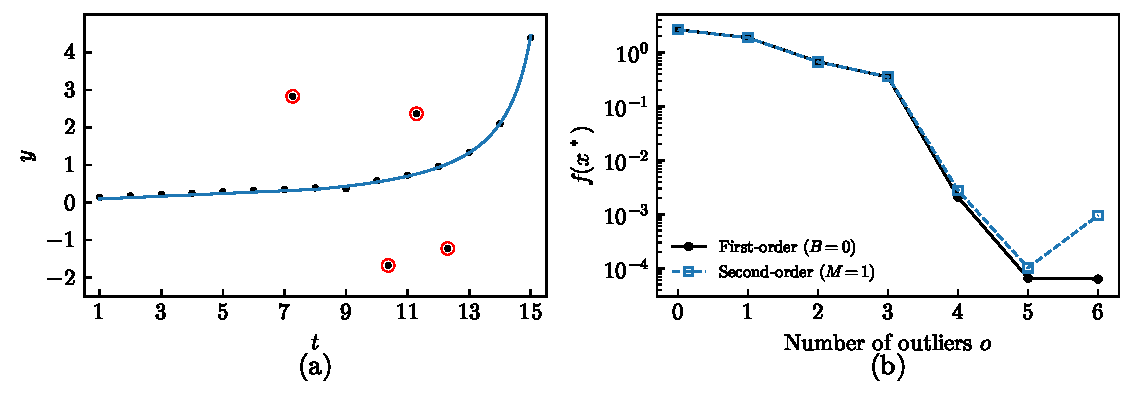
\includegraphics[width=\textwidth]{bard_panels.pdf}
\caption{Bard function with four added outliers, two above and two below the
model curve. (a) The fit returned at $o=4$ (solid line) follows the fifteen
clean observations (dots), while the four points identified as outliers
(circles) are discarded. (b) Best $f(x^*)$ over the $100$ starting points as a
function of the number $o$ of discarded observations, for both variants
(logarithmic vertical axis): $f(x^*)$ decreases only moderately up to $o=3$ and
drops by more than two orders of magnitude at $o=4$, after which it stays at the
residual floor of the clean data, the onset of which identifies the four
outliers.}
\label{fig:bard}
\end{figure}

Unlike the polynomial instance, the counts now differ between the two methods,
and the difference has structure. The aggregate over all $o$ is dominated by
$o = 0$---the minimax over all $m = 19$ observations, outliers included---a hard
nonconvex problem where both methods are expensive (about $360$--$400$ mean
iterations) and the first-order method is in fact slightly cheaper. Once at
least the outliers are being discarded ($o \ge 1$), the regime for which the
method is intended, the second-order variant uses fewer iterations and
evaluations in aggregate (but not less time; see Section~\ref{subsec:time}).
The comparison is not uniform row by row. The first-order method has the lower
mean iteration count at $o = 2$, $4$ and $6$, the lower mean evaluation count at
$o = 2$ and $6$, and the lower median iteration count at $o = 5$ and $6$. The
one metric that favors the second-order variant at every $o \ge 1$ is the median
evaluation count. Summing the per-$o$ means of Table~\ref{tab:bard} over
$o = 1, \dots, 6$ gives $232$ iterations and $296$ evaluations for the
first-order method against $134$ and $179$ for the second-order variant; the
corresponding sums of the per-$o$ medians are $43.5$ and $115$ against $40.5$
and $86$. The mean gap is sizeable---the first-order method uses about $1.7$
times as many iterations and evaluations---but it is driven by a heavy tail of
slow first-order runs at $o = 1$ (mean iteration count $152$ against $39$, with
medians $10.5$ and $7$), which the curvature mitigates. The medians, robust to
this tail, are much closer. In aggregate over this regime the curvature lowers
the iteration and evaluation counts, but the gain is moderate and is
concentrated in a few hard runs.

On this problem the curvature thus helps where the first-order model is a poor
local approximation, namely on a nonlinear model with outliers still present,
while it neither helps on the affine model of Section~\ref{subsec:poly} nor on the
full-data minimax at $o = 0$. This is consistent with the analysis of
Section~\ref{sec:complexity}, where the curvature affects only the constants of
the complexity bounds: any gain is a constant-factor one, not a change in the
order. Two caveats temper it. First, once the outliers are removed ($o \ge 4$)
both methods reach the residual floor of the clean data, where the first-order
variant attains the lower $f(x^*)$ values, by a factor of about $15$ at $o = 6$.
Second, the counts do not include the per-iteration cost of the curvature,
which is examined next.

\subsection{Computational cost} \label{subsec:time}

Iteration and evaluation counts do not reflect the extra work the second-order
variant performs at every iteration: for each active component it assembles the
Hessian $\nabla^2 f_i(x^k)$, diagonalizes it, applies the shift \eqref{shift}
and rescales it, at a cost of one \texttt{DSYEV} call per index in
$I_\delta(x^k)$. Table~\ref{tab:time} therefore reports CPU times, measured with
the Fortran intrinsic \texttt{cpu\_time} around the call to the algorithm and
aggregated in the same way as the counts: for each $o$ we take the mean and the
median over the $100$ starting points, and the table sums those per-$o$ values
over the sweep.

\begin{table}[ht!]
\centering
\begin{tabular}{l cc cc cc}
\hline
 & \multicolumn{2}{c}{First-order ($B=0$)}
 & \multicolumn{2}{c}{Second-order ($M=1$)}
 & \multicolumn{2}{c}{ratio} \\
\cline{2-3}\cline{4-5}\cline{6-7}
 & mean & median & mean & median & mean & median \\
\hline
Polynomial, $o=0,\dots,12$
  & $157.8$ & $147.4$ & $200.9$ & $186.1$ & $1.27$ & $1.26$ \\
Bard, $o=0,\dots,6$
  & $99.6$ & $66.1$ & $109.8$ & $63.3$ & $1.10$ & $0.96$ \\
Bard, $o=1,\dots,6$
  & $48.5$ & $15.5$ & $63.8$ & $17.1$ & $1.32$ & $1.10$ \\
\hline
\end{tabular}
\caption{CPU time in milliseconds for the polynomial of
Section~\ref{subsec:poly} and the Bard function of Section~\ref{subsec:bard},
summed over the sweep in $o$. For each $o$
the mean and median over the $100$ starting points are taken, as in
Tables~\ref{tab:poly} and~\ref{tab:bard}, and those values are then summed. The
ratio columns give second-order over first-order, so that values below $1$
favour the second-order variant.}
\label{tab:time}
\end{table}

On the polynomial, where the counts were indistinguishable, the
second-order variant costs about $27\%$ more time in the mean and in the
median: with nothing to gain from the curvature, building the matrices and
solving the subproblems with them is pure overhead. On the Bard problem the
iteration savings of Section~\ref{subsec:bard} do \emph{not} translate into
savings in time. Over the regime $o \ge 1$ the second-order variant is $32\%$
slower in the mean and $10\%$ slower in the median, and over the whole sweep it
is $10\%$ slower in the mean and $4\%$ faster in the median. The picture is
again not uniform: at $o = 1$, where the curvature shortens the heavy tail of
slow first-order runs, the second-order variant is about three times faster in
the mean ($4.7$ against $15.5$\,ms), but at $o = 2$, $4$ and $6$ it is slower,
both because its mean iteration counts are higher there and because each of its
iterations is more expensive. Since the typical run of either method
terminates in a handful of iterations, this per-iteration overhead is rarely
amortized. On problems of this size, the
reduction in iteration and evaluation counts obtained with the curvature should
therefore not be read as a reduction in computing time.

We note that these times are of the order of tens of milliseconds and, being
averages over $100$ runs of a single sweep, carry some machine noise; the
ratios, not the absolute values, are the meaningful quantity.

\subsection{Sensitivity to $\delta$ and $\sigma_{\min}$} \label{subsec:sens}

The band half-width $\delta$ and the initial regularization $\sigma_{\min}$ are
chosen by trial and error, so it is natural to ask how much of the above depends
on that choice. We repeated the Bard experiment of Section~\ref{subsec:bard} for
every combination of $\delta \in \{10^{-1},10^{-2},10^{-3},10^{-4}\}$ and
$\sigma_{\min} \in \{10^{-1},10^{-2},10^{-3}\}$, with $\gamma$, $\alpha$,
$\epsilon$, $M$ and the $100$ starting points unchanged, and with both methods.
Table~\ref{tab:sens} collects the results.

\begin{table}[ht!]
\centering
\resizebox{\textwidth}{!}{%
\begin{tabular}{cc ccc cc cc}
\hline
 & & & &
 & \multicolumn{2}{c}{First-order ($B=0$)}
 & \multicolumn{2}{c}{Second-order ($M=1$)} \\
\cline{6-7}\cline{8-9}
$\delta$ & $\sigma_{\min}$ & $f(x^*)$ at $o=3$ & $f(x^*)$ at $o=4$ & drop
 & \#it & \#fcnt & \#it & \#fcnt \\
\hline
$10^{-1}$ & $10^{-1}$ & 3.511e-01 & 2.086e-03 & $168\times$ & 232 & 296 & 134 & 179 \\
$10^{-1}$ & $10^{-2}$ & 3.536e-01 & 1.591e-03 & $222\times$ & 54 & 174 & 57 & 142 \\
$10^{-1}$ & $10^{-3}$ & 3.493e-01 & 1.813e-03 & $193\times$ & 36 & 183 & 77 & 192 \\
$10^{-2}$ & $10^{-1}$ & 3.491e-01 & 1.783e-03 & $196\times$ & 258 & 413 & 183 & 298 \\
$10^{-2}$ & $10^{-2}$ & 3.489e-01 & 1.350e-03 & $259\times$ & 83 & 339 & 124 & 331 \\
$10^{-2}$ & $10^{-3}$ & 3.489e-01 & 1.386e-03 & $252\times$ & 65 & 388 & 117 & 381 \\
$10^{-3}$ & $10^{-1}$ & 3.487e-01 & 1.327e-03 & $263\times$ & 332 & 684 & 247 & 529 \\
$10^{-3}$ & $10^{-2}$ & 3.488e-01 & 1.338e-03 & $261\times$ & 148 & 694 & 123 & 553 \\
$10^{-3}$ & $10^{-3}$ & 3.488e-01 & 1.329e-03 & $262\times$ & 110 & 727 & 127 & 648 \\
$10^{-4}$ & $10^{-1}$ & 3.487e-01 & 1.304e-03 & $267\times$ & 427 & 1158 & 375 & 982 \\
$10^{-4}$ & $10^{-2}$ & 3.487e-01 & 1.291e-03 & $270\times$ & 219 & 1249 & 179 & 940 \\
$10^{-4}$ & $10^{-3}$ & 3.487e-01 & 1.293e-03 & $270\times$ & 171 & 1286 & 181 & 1172 \\
\hline
\end{tabular}%
}
\caption{Sensitivity of the Bard experiment to $\delta$ and $\sigma_{\min}$.
The values of $f(x^*)$ and the drop factor between $o=3$ and $o=4$ are those of
the first-order method; the second-order variant agrees with them to within the
multistart variability. The count columns give the mean \#it and \#fcnt over the
$100$ starting points, summed over $o=1,\dots,6$. In all $24$ runs the $o=4$
solution identified exactly the four added outliers.}
\label{tab:sens}
\end{table}

Three things are stable across the table. The four outliers are identified
exactly in every one of the $24$ runs. The drop in $f(x^*)$ between $o=3$ and
$o=4$ is never smaller than two orders of magnitude, ranging from $168\times$ to
$270\times$. And the value of $f(x^*)$ at the plateau and at the floor varies
only in the third significant digit. The identification of the outliers, which
is what the method is used for, is therefore not an artefact of the particular
$\delta$ and $\sigma_{\min}$ reported in Section~\ref{subsec:bard}.

The counts, by contrast, do depend on the parameters. Decreasing $\delta$
raises the evaluation count steeply---at fixed $\sigma_{\min}=10^{-1}$, from
about $300$ at $\delta=10^{-1}$ to about $1200$ at $\delta=10^{-4}$ for the
first-order method---which is consistent with the threshold $9c_x^2/(2\delta)$
of Theorem~\ref{teo:suff-descent}: a narrower band forces a larger
$\sigma_{k,j}$, hence more rejected trial points per iteration. The effect of
$\sigma_{\min}$ on the iteration count is just as strong: at
$\delta = 10^{-1}$, decreasing $\sigma_{\min}$ from $10^{-1}$ to $10^{-3}$
reduces the mean iteration count of the first-order method from $232$ to $36$,
since a smaller initial regularization allows longer steps. The setting
$\delta=\sigma_{\min}=10^{-1}$ used in Section~\ref{subsec:bard}, inherited
from \cite{alvarezovo}, is in fact among the least favorable for the
first-order method; we keep it so that a single parameter set is used
throughout the paper.

The comparison between the two methods depends on $\sigma_{\min}$ in an
instructive way. The second-order variant has the lower mean evaluation count in
eleven of the twelve combinations, the exception being
$\delta=10^{-1}$, $\sigma_{\min}=10^{-3}$. Its advantage in iterations,
however, holds only when the initial regularization is large: it has the lower
mean iteration count in all four combinations with $\sigma_{\min}=10^{-1}$, in
two of the four with $\sigma_{\min}=10^{-2}$, and in none with
$\sigma_{\min}=10^{-3}$. Part of the benefit of the curvature reported in
Section~\ref{subsec:bard} is therefore a compensation for an over-regularized
first-order model: when $\sigma_{\min}$ is small, the first-order method already
takes long steps, and the curvature no longer reduces the number of iterations.

\subsection{An extended benchmark} \label{subsec:bench}

The two problems above are small and were chosen to isolate the effect of the
curvature. To assess the method on a broader and larger set, and to compare
different curvature families, we used the ten problems of the NIST Statistical
Reference Datasets for nonlinear regression \cite{nist} listed in
Table~\ref{tab:nist}. They cover exponential, rational and trigonometric models
with $n = 2$ to $9$ parameters and $m = 14$ to $250$ observations; each comes
with two official starting points and certified least-squares parameters. Each
data set was contaminated with outliers in two proportions, $5\%$ and $10\%$
of the observations (at least two). The contaminated observations were chosen
at random and displaced from their value, alternately upwards and downwards, by
$10$ times the residual standard deviation of the certified fit plus a random
fraction between $0.2$ and $0.4$ of the range of the fitted curve, so that
they are clearly separated from the noise of the clean data. Together with the
polynomial and Bard problems of Sections~\ref{subsec:poly}
and~\ref{subsec:bard}, this gives $22$ instances. The box $\Omega$ is the hull
of the two starting points and the certified parameters, enlarged by half of
their largest magnitude; for parameters that must keep their sign (rates,
widths, periods and denominator coefficients), the bound on the side of zero
is one tenth of the value closest to zero.

\begin{table}[ht!]
\centering
\small
\begin{tabular}{llrrrr}
\hline
Problem & Model class & $n$ & $m$ & \multicolumn{2}{c}{outliers} \\
\cline{5-6}
 & & & & $5\%$ & $10\%$ \\
\hline
Misra1a  & Exponential                  & 2 &  14 &  2 &  2 \\
Chwirut2 & Exponential                  & 3 &  54 &  3 &  5 \\
Rat43    & Exponential                  & 4 &  15 &  2 &  2 \\
MGH17    & Exponential (Osborne~1)      & 5 &  33 &  2 &  3 \\
Lanczos3 & Exponential                  & 6 &  24 &  2 &  2 \\
Thurber  & Rational (cubic/cubic)       & 7 &  37 &  2 &  4 \\
Kirby2   & Rational (quadratic/quadratic) & 5 & 151 &  8 & 15 \\
Bennett5 & Power                        & 3 & 154 &  8 & 15 \\
ENSO     & Trigonometric                & 9 & 168 &  8 & 17 \\
Gauss1   & Exponential with two peaks   & 8 & 250 & 12 & 25 \\
\hline
\end{tabular}
\caption{NIST nonlinear regression problems used in Section~\ref{subsec:bench},
with the number of outliers added in each of the two contamination levels.}
\label{tab:nist}
\end{table}

The method is used as in the previous sections. For each instance, each
official starting point is perturbed ten times (by a relative factor drawn
uniformly in $[-0.25, 0.25]$ per component, then projected onto $\Omega$), the
OVO problem is solved with $o$ equal to the number of added outliers, and the
best value is kept. A test problem is therefore a pair (instance, starting
point), and there are $42$ of them. A variant \emph{solves} a test problem when
the best value $f(x^*)$ of its ten runs that stopped at Step~5 is within a
relative tolerance of $10^{-3}$ of the best value found by any variant; its
cost is the total number of evaluations, or the total CPU time, of the ten
runs. We compare the first-order method with the three curvature families
described at the beginning of this section: the shifted Hessian and the
Gauss--Newton and shared BFGS matrices with $M = 10^4$, a value large enough
for the bound to be practically inactive, and the shifted Hessian with $M = 1$,
the configuration of the previous sections.

Table~\ref{tab:bench} summarizes the results and Figure~\ref{fig:profiles}
shows the performance profiles \cite{dolanmore} on the number of evaluations and
on the CPU time. Each variant performs $420$ runs. The per-instance results are
available with the code.

\begin{table}[ht!]
\centering
\small
\resizebox{\textwidth}{!}{%
\begin{tabular}{lcl cc cc cc}
\hline
Curvature & $M$ & norm control & solved & identified & \#fcnt ($10^6$) & CPU (min) & limit & safeguard \\
\hline
First-order & -- & -- & 26 & 35 & 2.49 & 28.6 & 4 & 30 \\
Shifted Hessian & $1$ & rescale & 31 & 36 & 2.67 & 64.8 & 6 & 25 \\
Shifted Hessian & $10^4$ & rescale & 25 & 31 & 8.90 & 197.4 & 79 & 22 \\
Gauss--Newton & $10^4$ & rescale & 25 & 32 & 2.86 & 41.2 & 4 & 22 \\
Shared BFGS & $10^4$ & rescale & 26 & 34 & 2.80 & 54.0 & 6 & 21 \\
\hline
\end{tabular}%
}
\caption{Extended benchmark ($42$ test problems, $420$ runs per variant).
\emph{solved}: test problems on which the best value of the multistart is
within $10^{-3}$ of the best value of any variant; \emph{identified}: test
problems on which the best run discards exactly the added outliers;
\#fcnt and CPU: totals over all runs; \emph{limit}: runs stopped by the
iteration or time limit; \emph{safeguard}: runs in which a trial point was
accepted after $100$ increases of $\sigma_{k,j}$. The CPU time of the shifted
Hessian with $M=1$ includes $30$ minutes charged to the single run in which
the subproblem solver failed to return (see the text); without it, the total
is $34.8$ minutes.}
\label{tab:bench}
\end{table}

\begin{figure}[ht!]
\centering
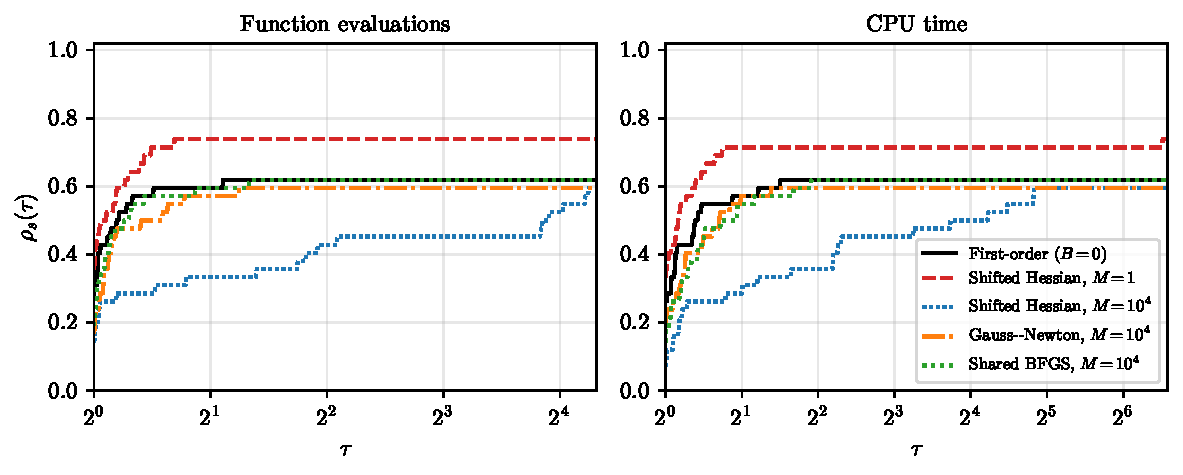
\includegraphics[width=\textwidth]{profiles.pdf}
\caption{Performance profiles on the extended benchmark ($42$ test problems).
$\rho_s(\tau)$ is the fraction of test problems that variant $s$ solves at a
cost at most $\tau$ times the smallest cost among the variants that solve it.
Left: total number of function evaluations of the multistart; right: total
CPU time.}
\label{fig:profiles}
\end{figure}

Three observations stand out. First, the shifted Hessian with $M=1$ is the most
robust variant: it solves $31$ of the $42$ test problems, against $26$ for the
first-order method, and identifies the outliers in $36$ of them, against $35$.
It reaches a strictly better minimizer than the first-order method on nine test
problems (Lanczos3, Kirby2, MGH17, Bennett5, ENSO and the polynomial) and a
worse one on four (Bard, Lanczos3 and MGH17). It is also the most efficient:
it has the smallest cost on $36\%$ of the test problems, against $29\%$ for the
first-order method, and a cost within twice the smallest on $74\%$, against
$60\%$. Its total cost exceeds that of the first-order method by $7\%$ in
evaluations and, excluding the failed run, by $22\%$ in CPU time.

Second, curvature without an effective bound is harmful. The shifted Hessian
with $M=10^4$ solves fewer test problems than the first-order method, uses
$3.6$ times as many evaluations, and stops at the iteration limit in $79$ runs,
mostly on Thurber, Rat43, Gauss1 and MGH17. On these problems the active set
contains components with large residuals, whose Hessians
$\nabla r_i\nabla r_i^T + r_i\nabla^2 r_i$ are strongly indefinite; the shift
\eqref{shift} then adds a large multiple of the identity, which acts as an
additional regularization and shortens the steps. Section~\ref{subsec:M}
examines this effect.

Third, the Gauss--Newton and shared BFGS matrices, which need no shift, behave
much like the first-order method: they solve $25$ and $26$ test problems at a
cost $12$--$15\%$ higher in evaluations. On the well-scaled problems (Chwirut2,
ENSO, Gauss1) all variants reach the same minimizers at similar costs.

Overall, the extended benchmark confirms and qualifies the picture of the
previous sections. A suitably bounded curvature improves the robustness of the
multistart and, on several problems, the quality of the minimizer found, at a
moderate cost; but the benefit depends on the problem and on how the size of
the curvature is controlled, and no variant dominates the others on every
problem. Section~\ref{subsec:M} shows that a bound proportional to the
regularization parameter retains this robustness at a lower cost.

Regarding the safeguards, the iteration limit was reached in $4$ to $11$ runs
per variant, except for the shifted Hessian with $M=10^4$ ($79$ runs) and with
$M=10$ under eigenvalue clipping ($38$ runs; Section~\ref{subsec:M}), and the
inner-loop safeguard was activated in $21$ to $41$ runs per variant, always
once $\|x^{k,j}_{\mathrm{trial}} - x^k\|$ had become negligible. In a single run
out of the $4620$ of this section (Gauss1, shifted Hessian, $M=1$), Algencan
failed to return from one subproblem; that run is counted as unsuccessful and
charged with a CPU time of $30$ minutes.


\emph{Cost and size of the active set.} With $\delta = 0.1$, the active sets
of the benchmark are small, even when $m$ is large: on the four largest
instances, $I_\delta(x^k)$ contains on average between $4$ and $51$
components. To study the cost when the active set is large, we reran these
instances (contamination level $10\%$, first starting point, ten runs) with
$\delta \in \{10^{-1}, 1, 10, 10^2, 10^3\}$, which increases the mean size of
$I_\delta(x^k)$ up to the whole set of observations. Table~\ref{tab:active}
reports the CPU time per subproblem, that is, the total CPU time divided by the
number of trial points, each of which requires one subproblem and one
evaluation of $f$.

\begin{table}[ht!]
\centering
\small
\resizebox{\textwidth}{!}{%
\begin{tabular}{llr ccc cc}
\hline
 & & & \multicolumn{3}{c}{ms per subproblem} & \multicolumn{2}{c}{ratio to first-order} \\
\cline{4-6}\cline{7-8}
Problem & $\delta$ & $|I_\delta|$ & First-order & Shifted Hessian & Gauss--Newton
 & Shifted Hessian & Gauss--Newton \\
\hline
Bennett5 & $10^{-1}$ & 50.7 & 5.33 & 5.63 & 5.63 & 1.06 & 1.06 \\
 & $10^{0}$ & 92.3 & 0.91 & 0.98 & 1.00 & 1.08 & 1.10 \\
 & $10^{1}$ & 121.2 & 1.05 & 1.28 & 1.25 & 1.21 & 1.19 \\
 & $10^{2}$ & 154.0 & 1.09 & 1.19 & 1.31 & 1.10 & 1.20 \\
 & $10^{3}$ & 154.0 & 1.06 & 1.17 & 1.31 & 1.10 & 1.23 \\
Kirby2 & $10^{-1}$ & 7.2 & 2.47 & 2.72 & 2.76 & 1.10 & 1.12 \\
 & $10^{0}$ & 22.3 & 1.23 & 2.16 & 1.95 & 1.76 & 1.59 \\
 & $10^{1}$ & 33.7 & 2.22 & 3.91 & 2.70 & 1.76 & 1.21 \\
 & $10^{2}$ & 33.8 & 1.47 & 1.93 & 1.22 & 1.31 & 0.83 \\
 & $10^{3}$ & 84.8 & 3.32 & 5.76 & 1.57 & 1.74 & 0.47 \\
ENSO & $10^{-1}$ & 4.5 & 0.46 & 0.49 & 0.47 & 1.06 & 1.03 \\
 & $10^{0}$ & 5.6 & 0.49 & 0.50 & 0.52 & 1.04 & 1.07 \\
 & $10^{1}$ & 13.4 & 0.87 & 1.66 & 0.75 & 1.92 & 0.87 \\
 & $10^{2}$ & 151.2 & 14.96 & 21.09 & 26.98 & 1.41 & 1.80 \\
 & $10^{3}$ & 168.0 & 11.39 & 5.28 & 5.65 & 0.46 & 0.50 \\
Gauss1 & $10^{-1}$ & 4.1 & 1.08 & 1.11 & 1.10 & 1.03 & 1.02 \\
 & $10^{0}$ & 5.3 & 1.39 & 1.22 & 1.38 & 0.88 & 1.00 \\
 & $10^{1}$ & 7.3 & 2.19 & 2.16 & 1.80 & 0.98 & 0.82 \\
 & $10^{2}$ & 10.8 & 1.82 & 10.66 & 9.75 & 5.86 & 5.37 \\
 & $10^{3}$ & 109.4 & 14.74 & 27.97 & 15.26 & 1.90 & 1.04 \\
\hline
\end{tabular}%
}
\caption{CPU time per subproblem as the band half-width $\delta$ increases, on
the four largest instances ($10\%$ of outliers, first starting point, ten
runs; curvature matrices with $M=1$). $|I_\delta|$ is the mean size of the
active set over the iterations of the first-order runs. For the shifted
Hessian on Gauss1 with $\delta = 10^{-1}$, the run in which the subproblem
solver failed is excluded.}
\label{tab:active}
\end{table}

Two observations follow. First, the cost per subproblem grows with the size of
the active set for all variants, and it also depends on $n$. On ENSO ($n=9$) and
Gauss1 ($n=8$) it rises from $0.5$--$1.4$\,ms with a handful of active
components to $5$--$28$\,ms with more than one hundred. On Bennett5 ($n=3$) it
stays close to $1$\,ms even with all $154$ observations active; the higher
value at $\delta = 10^{-1}$ reflects harder subproblems rather than a larger
set. This cost, common to all variants, comes from the solution of the
subproblem, whose number of constraints is $|I_\delta(x^k)|$. Second, the
overhead of the curvature per subproblem does not grow with the size of the
active set. Over the twenty settings, the median ratio to the first-order
method is $1.10$ for the shifted Hessian and $1.07$ for the Gauss--Newton
matrix. The largest ratios (up to $5.9$, on Gauss1 with $\delta = 10^2$)
correspond to settings in which the subproblems with curvature require more
work from the solver, not to larger active sets. Since $n \leq 9$ here,
building the curvature matrices (one eigenvalue decomposition per active
component for the shifted Hessian) is cheap compared with solving the
subproblem. For larger $n$, the $O(n^3)$ cost per active component would
become significant; the Gauss--Newton matrix, whose norm is
$\|\nabla r_i\|^2$ and which needs no decomposition, or a matrix shared by all
components, would then be preferable.

\subsection{The role of the bound $M$} \label{subsec:M}

The bound $\|B_{k,j,i}\|\le M$ is essential in the analysis, and the
experiments above show that it is also decisive in practice. We first discuss
what the theory says about it, and then report a sensitivity experiment.

\emph{What the theory says.} The constant $M$ enters the iteration bound
\eqref{cota-iter} only through the factor $(M + \sigma_{\max})^2$, where
$\sigma_{\max} \geq \gamma(L + 2\alpha) > L$. Any choice $M \leq \sigma_{\max}$
therefore increases this factor by at most $4$ with respect to the first-order
method. Moreover, under Assumption~\ref{a4} the Hessians of twice
continuously differentiable components satisfy $\|\nabla^2 f_i\| \leq L$, so
the shifted Hessian \eqref{shift} has norm at most $2L + \tau$: the choice
$M = 2L + \tau$ makes the bound inactive for exact Hessians at the price of a
constant factor in \eqref{cota-iter}. The theory thus gives no reason to
prefer a small $M$; it only requires $M$ to be bounded. It also allows $M$ to
vary, as long as it remains bounded: since Step~2 chooses $B_{k,j,i}$ after
$\sigma_{k,j}$ is known, the adaptive rule $\|B_{k,j,i}\| \leq c\,\sigma_{k,j}$,
with a fixed $c > 0$, is admissible with $M = c\,\sigma_{\max}$, and keeps the
size of the curvature proportional to that of the regularization.

\emph{Sensitivity experiment.} We repeated the benchmark of
Section~\ref{subsec:bench} with the shifted Hessian for
$M \in \{0.1, 1, 10, 10^2, 10^4\}$, with eigenvalue clipping (eigenvalues larger
than $M$ are replaced by $M$, the eigenvectors being kept) instead of rescaling
for $M \in \{1, 10\}$, and with the Gauss--Newton matrix for $M = 1$. We also
tested the adaptive bound $\|B_{k,j,i}\| \le c\,\sigma_{k,j}$ with
$c \in \{1, 10, 10^2\}$: the shifted Hessian is computed once per outer
iteration and, for each value of $\sigma_{k,j}$ tried in the inner loop,
rescaled by $\min\{1, c\,\sigma_{k,j}/\lambda_{\max}(B_{k,j,i})\}$.
Table~\ref{tab:M} reports the results; a test problem is now counted as solved
when the variant attains the best value among all fourteen variants.

\begin{table}[ht!]
\centering
\small
\resizebox{\textwidth}{!}{%
\begin{tabular}{lcl cc cc cc}
\hline
Curvature & $M$ & norm control & solved & identified & \#fcnt ($10^6$) & CPU (min) & limit & safeguard \\
\hline
First-order & -- & -- & 20 & 35 & 2.49 & 28.6 & 4 & 30 \\
Shifted Hessian & $0.1$ & rescale & 17 & 34 & 4.38 & 49.6 & 11 & 22 \\
Shifted Hessian & $1$ & rescale & 25 & 36 & 2.67 & 64.8 & 6 & 25 \\
Shifted Hessian & $10$ & rescale & 19 & 33 & 2.75 & 28.2 & 5 & 21 \\
Shifted Hessian & $10^2$ & rescale & 23 & 32 & 4.32 & 59.1 & 8 & 33 \\
Shifted Hessian & $10^4$ & rescale & 20 & 31 & 8.90 & 197.4 & 79 & 22 \\
Shifted Hessian & $1$ & clip & 21 & 35 & 4.94 & 71.8 & 6 & 41 \\
Shifted Hessian & $10$ & clip & 19 & 33 & 6.13 & 94.5 & 38 & 35 \\
Shifted Hessian & $\sigma_{k,j}$ & adaptive & 20 & 37 & 2.18 & 18.7 & 3 & 26 \\
Shifted Hessian & $10\,\sigma_{k,j}$ & adaptive & 23 & 37 & 2.47 & 21.3 & 9 & 17 \\
Shifted Hessian & $10^2\sigma_{k,j}$ & adaptive & 20 & 35 & 4.12 & 77.6 & 21 & 17 \\
Gauss--Newton & $1$ & rescale & 21 & 36 & 2.76 & 38.0 & 4 & 22 \\
Gauss--Newton & $10^4$ & rescale & 21 & 32 & 2.86 & 41.2 & 4 & 22 \\
Shared BFGS & $10^4$ & rescale & 19 & 34 & 2.80 & 54.0 & 6 & 21 \\
\hline
\end{tabular}%
}
\caption{Sensitivity to $M$ and to the norm control on the extended benchmark
($42$ test problems). Columns as in Table~\ref{tab:bench}; a test problem is
solved when the best value of the multistart is within $10^{-3}$ of the best
value of any of the fourteen variants. For the adaptive bound, the column $M$
gives the bound on $\|B_{k,j,i}\|$ in terms of $\sigma_{k,j}$.}
\label{tab:M}
\end{table}

Five conclusions can be drawn.
\begin{itemize}
\item \emph{With a fixed bound, the shifted Hessian is sensitive to $M$, and not
monotonically.} Among the fixed bounds, $M = 1$ gives the most robust variant
and the smallest number of evaluations; only $M = 10$ is slightly cheaper in
CPU time, at a clear loss in robustness. With large $M$ the shift dominates and the cost grows sharply.
With $M = 0.1$ the variant is less robust and more expensive than the
first-order method itself. We do not have a complete explanation for this
case; it shows, at least, that a small bound does not simply reduce the method
to its first-order counterpart.
\item \emph{Rescaling preserves more information than clipping.} Rescaling
keeps the eigenvectors and the ratios between eigenvalues and only changes the
magnitude of the matrix. When the shift in \eqref{shift} is large, all
eigenvalues of the shifted matrix are large, so clipping replaces the matrix by
approximately $M I$, which carries no directional information and acts as an
additional regularization. Accordingly, clipping is no more robust than
rescaling and $1.8$ to $2.3$ times more expensive for the same $M$.
\item \emph{The Gauss--Newton matrix is insensitive to $M$.} It needs no
shift, and the results for $M=1$ and $M=10^4$ are almost identical in
robustness and cost.
\item \emph{Rescaling does distort the curvature when $\|B_{k,j,i}\| \gg M$.}
For instance, on the polynomial of Section~\ref{subsec:poly} it reduces the
curvature by up to three orders of magnitude. Nevertheless, a bounded,
rescaled curvature performed better than an unbounded one in our tests.
\item \emph{The adaptive bound is the most efficient choice.} With $c = 10$, it
solves $23$ test problems, second only to the fixed bound $M = 1$ ($25$),
identifies the outliers in $37$, as many as with $c = 1$ and more than any
other variant, and does so with
$2.47 \times 10^6$ evaluations and $21.3$ minutes of CPU time, that is, at a
lower cost than the first-order method ($2.49 \times 10^6$ evaluations and
$28.6$ minutes) and than any fixed bound. With $c = 1$ it is the cheapest
variant of all ($2.18 \times 10^6$ evaluations, $18.7$ minutes), with the
robustness of the first-order method. With $c = 10^2$ it behaves like a large
fixed bound. Compared only with the first-order method and the fixed bound
$M = 1$, the adaptive bound with $c = 10$ solves $28$ of the $42$ test
problems, as many as $M = 1$ and against $22$ for the first-order method.
\end{itemize}

In practice, the role of $M$ is to cap the weight of the curvature relative to
the regularization, and the adaptive bound makes this explicit. With
$c = 10$, the bound coincides with the best fixed value $M = 1$ at the start of
each inner loop, where $\sigma_{k,0} = \sigma_{\min} = 0.1$, and then grows
with $\sigma_{k,j}$: when the regularization has to be increased, the
curvature is allowed to increase with it, instead of becoming negligible. This
choice needs no tuning to the scale of the problem, since $\sigma_{k,j}$ itself
adapts to it, and it is admissible in the theory with
$M = c\,\sigma_{\max}$. We therefore recommend it over a fixed $M$ chosen by
trial and error. It is the only configuration in our experiments in which the
curvature reduces the CPU time appreciably with respect to the first-order
method.

Finally, the margin $\tau$ in \eqref{shift} has no noticeable effect. On the
Bard experiment of Section~\ref{subsec:bard}, the values
$\tau \in \{0, 10^{-8}, 10^{-4}\}$ give the same iteration and evaluation counts
up to $0.4\%$ and essentially the same solutions, and $\tau = 10^{-2}$
increases the
iteration count by $4.5\%$, the four outliers being identified in all cases.


\section{Final remarks} \label{sec:final}

We have extended the first-order regularized method of \cite{alvarezovo} for
box-constrained order-value optimization by enriching its model with curvature,
each active component carrying its own positive semidefinite matrix of norm at
most $M$. The resulting method is well defined and, under standard smoothness
assumptions and without any assumption on the Lagrange multipliers of the
subproblems (Lemma~\ref{lem:step}), attains worst-case iteration- and
evaluation-complexity bounds of the same order as its first-order counterpart
(Theorem~\ref{teo:complexity}), of which it is a strict generalization; the curvature enters only through the
constant $M$ in \eqref{cota-iter}, and not through the order of the bound. The
curvature is thus accommodated at no cost in the order of the theoretical
guarantees. Positive semidefiniteness and the bound $M$ are the only
requirements imposed on the matrices, so quasi-Newton updates such as BFGS or
SR1, Gauss--Newton matrices and shifted exact Hessians all fit directly into the
framework; individual positive semidefiniteness is used in
Theorem~\ref{teo:suff-descent} to make the model an upper approximation of each
active component, while only the convex combination $\bar{B}_{k,j}$ of
Corollary~\ref{cor:step} enters the complexity bound.

The numerical experiments support a conditional conclusion: the curvature
helps when the first-order model is a poor local approximation and the size of
the curvature is suitably controlled, and it is neutral or harmful otherwise.
On the affine polynomial model the curvature is redundant and only adds cost.
On the nonlinear Bard model, once outliers are being discarded, it reduces the
iteration and evaluation counts by a factor of about $1.7$ in the mean, mainly
by curbing a heavy tail of slow first-order runs, but this does not translate
into a shorter CPU time, and the advantage in iterations disappears when the
first-order method is run with a small initial regularization
(Section~\ref{subsec:sens}). On the broader benchmark of
Section~\ref{subsec:bench}, the shifted Hessian with $M=1$ is the most robust
variant, solving $31$ of $42$ test problems against $26$ for the first-order
method at a similar cost, while the same matrices without an effective bound
are by far the most expensive, and the Gauss--Newton and BFGS matrices behave
much like the first-order method. Section~\ref{subsec:M} shows that $M$ is a
decisive parameter: it caps the weight of the curvature relative to the
regularization. An adaptive bound proportional to the regularization
parameter, $\|B_{k,j,i}\| \le 10\,\sigma_{k,j}$, which is covered by the theory
and needs no tuning, is nearly as robust as the best fixed bound and is the
only configuration in which the curvature reduced the CPU time appreciably
with respect to the first-order method. These findings are consistent with the complexity analysis, in
which the curvature affects only the constant of the bound and not its order:
what can be expected from the curvature is a constant-factor gain, in
efficiency or in the quality of the minimizer reached, on suitable problems,
not a uniform improvement. The experiments also show that the constant of the
worst-case bound is not a guide to practical performance: with the adaptive
bound, the factor $(M + \sigma_{\max})^2 = (1 + c)^2\sigma_{\max}^2$ in
\eqref{cota-iter} grows with $c$, yet $c = 10$ was more robust than $c = 1$.
The bound describes the worst case, whereas the practical value of the
curvature depends on the behavior far from it.

Compared with the quasi-Newton method of \cite{yano1}, the present method trades
asymptotic local rates for non-asymptotic global guarantees
(Section~\ref{sec:complexity}). The method of \cite{yano1} attains superlinear and
quadratic local convergence under isolation and nondegeneracy assumptions, but
gives no bound on the work needed to reach approximate stationarity. The
present method gives such bounds under global assumptions only, but no local
rate has been established for it, and with Hessian-like curvature its
regularization, bounded below by $\sigma_{\min}$, perturbs the Newton step.
Letting the regularization decrease across iterations, as suggested for the
first-order method in \cite{alvarezovo}, or choosing the curvature matrices to
compensate for it, are natural ways to seek both properties at once.

The reason the curvature does not change the order is structural. The Tikhonov
term $\sigma\|x - \bar x\|^2$ makes the model an upper approximation of $f$ once
$\sigma$ is of order $L$, which bounds the accepted step from below by a
multiple of $\epsilon$ at every iteration at which the stopping test fails,
hence a per-iteration decrease of order $\epsilon^2$ and the $O(\epsilon^{-2})$
iteration bound. A natural way to
genuinely improve the order is to replace the quadratic regularization by a
cubic one, $\tfrac{\sigma}{3}\|x - \bar x\|^3$, in the spirit of the
cubic-regularization method of \cite{nesterov} and the high-order regularized
models of \cite{bgmst1, bgms}. With accurate second-order information---the true
or Gauss--Newton Hessian of each active component, used unmodified rather than
shifted and rescaled to meet an arbitrary bound $M$---and under the additional
assumption that the component Hessians are
Lipschitz continuous, the cubic model is an upper approximation with a step of
size $O(\epsilon^{1/2})$ and a per-iteration decrease of order $\epsilon^{3/2}$,
which would improve the iteration bound to $O(\epsilon^{-3/2})$. Realizing this
for the order-value function is not a direct transfer: the objective is
nonsmooth, the complexity carries the two parameters $\delta$ and $\epsilon$, and
the approximate optimality condition $C_{\delta,\epsilon}$ is stated in terms of
active gradients. Extending the analysis to a cubically regularized model,
tracking the interaction of the improved $\epsilon$-dependence with $\delta$, is
a promising direction in which the curvature would acquire a provable role, at
the price of a stronger smoothness assumption, accurate second-order information,
and a cubically regularized subproblem.

\section*{Declarations}

\medskip
\noindent
\textbf{Funding.} This work was funded by the Vice-Rectorate for Research, Outreach and Social Projection of the University of the Atlantic through the 2022 Internal Call for Proposals to Strengthen Research Groups with Tools for Creation, Innovation, and Research (award code CB734-CII2023).

\medskip
\noindent
\textbf{Conflicts of interest.} The authors have no relevant financial or non-financial interests to disclose.

\medskip
\noindent
\textbf{Data and code availability.} The polynomial data set of Section~\ref{subsec:poly} is the one of \cite{dunder1}. The data of Section~\ref{subsec:bard} consist of the 15 observations of the Bard function listed in \cite{mgh} together with four outliers generated with a fixed random seed, as described there. The data of Section~\ref{subsec:bench} are the NIST Statistical Reference Datasets for nonlinear regression \cite{nist}, contaminated with outliers by a script with a fixed random seed. The Fortran 90 implementation of Algorithm~\ref{alg:main} (including all curvature families and norm controls), all data sets, the per-instance results, and the scripts that reproduce every table and figure of Section~\ref{sec:numerical} are openly available at \url{https://github.com/gdquintero/ovoqnewton}.

\medskip
\noindent
\textbf{Authors' contributions.} All authors contributed to the conception and design of the study, to the analysis, and to the writing of the manuscript. All authors read and approved the final manuscript.

\medskip
\noindent
\textbf{Acknowledgements.} The authors thank the University of the Atlantic and its Vice-Rectorate for Research, Outreach and Social Projection for granting access to the Centro de Modelación Matemática.

\clearpage

\begin{thebibliography}{99}

\bibitem{dunder1} R. Andreani, C. Dunder and J. M. Mart\'{\i}nez, Order-Value Optimization: Formulation and solution by means of a primal Cauchy method, \textit{Mathematical Methods of Operations Research} 58, pp. 387--399, 2003.

\bibitem{dunder2} R. Andreani, C. Dunder and J. M. Mart\'{\i}nez, Nonlinear-programming reformulation of the order-value optimization problem, \textit{Mathematical Methods of Operations Research} 61, pp. 365--384, 2005.

\bibitem{yano1} R. Andreani, J. M. Mart\'{\i}nez, M. Salvatierra, and F. S. Yano, Quasi-Newton methods for Order-Value Optimization and Value-at-Risk calculations, \textit{Pacific Journal of Optimization} 2, pp. 11--33, 2006.

\bibitem{yano2} R. Andreani, J. M. Mart\'{\i}nez, L. Mart\'{\i}nez, and F. S. Yano, Low order-value optimization and applications, \textit{Journal of Global Optimization} 43, pp. 1--22, 2009.

\bibitem{salva} R. Andreani, J. M. Mart\'{\i}nez, M. Salvatierra, and F. S. Yano, Global order-value optimization by means of a multistart harmonic oscillator tunneling strategy, in \textit{Global Optimization: From Theory to Implementation}, L. Liberti and N. Maculan (eds.), Springer, Boston, MA, 2006, pp. 379--404.

\bibitem{bgms} E. G. Birgin, J. L. Gardenghi, J. M. Mart\'{\i}nez, and S. A. Santos, On the use of third-order models with fourth-order regularization for unconstrained optimization, \textit{Optimization Letters} 14, pp. 815--838, 2020.

\bibitem{bgmst2} E. G. Birgin, J. L. Gardenghi, J. M. Mart\'{\i}nez, S. A. Santos, and Ph. L. Toint, Evaluation complexity for nonlinear constrained optimization using unscaled KKT conditions and high-order models, \textit{SIAM Journal on Optimization} 26, pp. 951--967, 2016.

\bibitem{bgmst1} E. G. Birgin, J. L. Gardenghi, J. M. Mart\'{\i}nez, S. A. Santos, and Ph. L. Toint, Worst-case evaluation complexity for unconstrained nonlinear optimization using high-order regularized models, \textit{Mathematical Programming} 163, pp. 359--368, 2017.

\bibitem{bmbook} E. G. Birgin and J. M. Mart\'{\i}nez, \textit{Practical Augmented Lagrangian Methods for Constrained Optimization}, Society for Industrial and Applied Mathematics, Philadelphia, 2014.

\bibitem{bmcomper} E. G. Birgin and J. M. Mart\'{\i}nez, Complexity and performance of an Augmented Lagrangian algorithm, \textit{Optimization Methods and Software} 35, pp. 885--920, 2020.

\bibitem{cogtbook} C. Cartis, N. I. M. Gould, and Ph. L. Toint, \textit{Evaluation Complexity of Algorithms for Nonconvex Optimization: Theory, Computation, and Perspectives}, SIAM, Philadelphia, PA, 2022.

\bibitem{dolanmore} E. D. Dolan and J. J. Mor\'e, Benchmarking optimization software with performance profiles, \textit{Mathematical Programming} 91, pp. 201--213, 2002.

\bibitem{gauvin} J. Gauvin, A necessary and sufficient regularity condition to have bounded multipliers in nonconvex programming, \textit{Mathematical Programming} 12, pp. 136--138, 1977.

\bibitem{jorion} P. Jorion, \textit{Value at {R}isk: {T}he new benchmark for managing financial risk}, 3rd. ed., McGraw-Hill, 2009.

\bibitem{mtop} J. M. Mart\'{\i}nez, Generalized Order-Value Optimization, \textit{TOP} 20, pp. 75--98, 2012.

\bibitem{mgh} J. J. Mor\'e, B. S. Garbow, and K. E. Hillstrom, Testing unconstrained optimization software, \textit{ACM Transactions on Mathematical Software} 7, pp. 17--41, 1981.

\bibitem{nist} National Institute of Standards and Technology, \textit{Statistical Reference Datasets: Nonlinear Regression}, \url{https://www.itl.nist.gov/div898/strd/nls/nls_main.shtml}.

\bibitem{nesterov} Y. Nesterov and B. T. Polyak, Cubic regularization of Newton method and its global performance, \textit{Mathematical Programming} 108, 177--205, 2006.

\bibitem{jiang} Z. Jiang, Q. Hu, and X. Zheng, Optimality condition and complexity of order-value optimization problems and low order-value optimization problems, \textit{Journal of Global Optimization} 69, pp. 511--523, 2017.

\bibitem{alvarezovo} G. Q. Álvarez and E. G. Birgin, A first-order regularized approach to the order-value optimization problem, \textit{Optimization Methods and Software} 40, pp. 650--674, 2025.
    
\end{thebibliography}

\end{document}